\part{État de l'art}
Dans nos recherches sur la gestion de flux de données pour l'observation des systèmes, nous avons été amenés à étudier de nombreux travaux. Sans vouloir être exhaustifs, nous consacrons ici un chapitre à diverses solutions orientées\textit{observation et analyse de systèmes} sans que forcément elles intègrent des flux de données. Chacune des solutions présentées permet de répondre à une partie des problématiques. En complément, nous présentons un deuxième chapitre consacré à la \textit{gestion de flux de données} sans que forcément elle soit intégrée à une solution d'observation des systèmes.

\chapter{Gestion de données pour l'observation}
\minitoc

La supervision est un domaine très actif du fait de ses implications concrètes. Plusieures solutions ont déjà été proposées pour résoudre les différentes problématiques détaillées en section~\ref{sec:intro:problematique}. En dehors des systèmes d'observations ad-hoc qui ne peuvent pas répondre à l'hétérogénéité conséquente à laquelle cette thèse fait face, plusieurs approches ont étés développées. Ce chapitre présente les quatre grandes familles que nous avons pu identifier. Toutes ces approches sont capables de gérer les données issues d'un système générique.

Les critères qui nous permettrons de qualifié les différentes approches selon notre problématique seront développés dans la première section. Puis nous décrirons les quatres approches que nous avons analysées. Tout d'abord, en section~\ref{sec:rw:supervision:administration}, nous présenterons les systèmes d'administrations. Ceux-ci sont déployés depuis plusieurs années pour permettre de gérer des parcs de dispositifs à grandes échelles. Puis nous détaillerons la gestion de contexte en section~\ref{sec:rw:supervision:contexte}. Ces systèmes permettent de fournir à une architecture logicielle des informations de contexte pour qu'elle puisse s'adapter en conséquence. Les moyens pour représenter et manipuler les données sont très génériques. Puis nous développerons l'approche par entrepôts de données en section~\ref{sec:rw:supervision:warehouse}. Les entrepôts sont maintenant largement répandus et réputés pour avoir de grandes capacités d'analyses sur un ensemble de données intégré de manière hétérogène. Enfin, nous présenterons les systèmes de gestions de flux de données en section~\ref{sec:rw:supervision:datastream}. Ces systèmes permettent eux de manipuler des flux de données très dynamiques de manière déclarative.

Ces systèmes sont donc candidats pour permettre de créer un système d'observation générique.

\section{Critères d'analyse}
\TODO{Intro}
\subsection{Structure des données}
Cette thèse suppose que les données sont accessibles au dessus d'une couche d'abstraction. Cependant, aucune hypothèse n'a été formulée sur la structure de ces données ou leurs formats. Ce premier critère d'analyse se focalise donc sur le formalisme utilisé lors de l'acquisition des données. Trois sous-critères sont décrit : la structure abstraite, la gestion de l'hétérogénéité sémantique et enfin le support de l'évolution des données.

\subsubsection{Structure abstraite}
Un modèle de données abstrait permet de décrire une représentation d'un ensemble de données de façon abstrait. Des exemples classiques de ce type de modèles sont : relationnel, objet, sémantique, à dimension ou encore hiérarchique. Ce modèle abstrait permettra par la suite de définir tout autant la capacité de représentation des données que ses capacités intrinsèques en terme de traitement. Ainsi, le choix de cette structure sera central pour la gestion de l'hétérogénéité.
\subsubsection{Sémantique}
Une donnée est liée à différents concepts. La capacité à représenter ces liens sémantiques est primordiale afin de gérer un grand ensemble de données. Si une telle distinction est explicitement faite, il sera possible de différencier à quel(s) concept(s) appartient une donnée. Ceci permet de lever des ambiguïtés telle que l'attachement de la donnée \textit{Statut}. Ce paramètre a en effet un sens différent suivant son attachement : \textit{Équipement}, \textit{Application} ou \textit{Service}. Le lien entre les différents concepts permet aussi de pouvoir annoter les données avec des meta-informations qui permettrons d'adapter le traitement par la suite.
\subsubsection{Dynamisme}
La valeur obtenue à un instant particulier d'une donnée n'est pas toujours relevant. En effet, pour plusieurs types d'informations, la pertinence de la donnée va être accordé à son évolution au fur et à mesure du temps. Les différents types de dynamiques ont étés présentés en section~\ref{sec:intro:problematique:data}. La capacité à ce modèle d'être capable de représenter les différentes évolutions sera critique à l'intégration des différentes sources de données hétérogènes.

\subsection{Traitement}
Afin d'évaluer la capacité du système de supervision à fournir les réponses les plus précises à l'utilisateur, il faut établir des processus de traitements sur les données. Suivant les systèmes, cette capacité à collecter et transformer les données des sources n'a pas la même puissance. Ainsi, il est nécessaire d'analyser plus en profondeur les capacités de ce procédé. Nous détaillerons ceci en quatre critères principaux : les types d'interrogation possibles, l'intégration de sources, le langage d'expression et enfin le pouvoir expressif de ce langage.

\subsubsection{Types d'interrogations}
La création des processus de traitements de données est assimilable à une interrogation que pose l'utilisateur sur l'ensemble des données. Il existe différentes natures d'interrogations (ou requêtes). Celles-ci reflètent l'hétérogénéité de la dynamique des données.
\begin{itemize}
    \item \textbf{Interrogation instantanée} : il constitue le paradigme usuel d'interrogation utilisé notamment dans les applications de gestion de base de données. L'utilisateur pose une question sur un ensemble de données considérées figées du moins le temps du calcul de la réponse. Le système fournit une réponse figée elle aussi. Un exemple simple étant : ``quel est l'ensemble actuel des capteurs de température de mon système''. La réponse sera ``à cet instant, les capteurs 1, 4 et 42 sont des capteurs de température du système''. La mention ``à cet instant'' est très importante car si un nouveau capteur arrive dans le système, la réponse deviendra erronée. Il est bien évidemment possible d'imaginer revenir dans le passé et poser une question sur un état antérieur. La consultation ponctuelle de l'ensemble de données par l'utilisateur est donc une application de cette interrogation.
    \item \textbf{Interrogation continue} : principal acteur des systèmes événementiels, ce paradigme considère que les données sont en constante évolution. L'utilisateur obtiendra ainsi une réponse qui évoluera au cours du temps, sous forme de flux ou de mise à jour d'état. Un exemple pouvant être : ``quel est la température moyenne sur une minute du capteur 42''. La réponse sera un flux continu d'information qui, toutes les minutes, reportera une nouvelle valeur moyenne pour ce capteur. Ainsi, la formation de processus de collecte ou de formation d'alerte sont des applications de ce type d'interrogation.
\end{itemize}
Il est important de noter que ces deux grands paradigmes d'interrogation peuvent se combiner. Par exemple, il est possible d'effectuer un appel à une interrogation instantanée à l'intérieur d'un processus continu. Il est donc nécessaire que le système d'observation soit capable de manipuler naturellement ces deux types d'interrogations pour manipuler correctement le dynamisme des données.

\subsubsection{Intégration de sources}
Pour permettre une grande compréhension du système et de ses interactions, il est nécessaire de corréler les différentes sources d'informations en une seule base d'information intégrée. En effet, chaque source de donnée peut-être considérée comme un fragment de cette ensemble intégré. Ainsi, il est nécessaire que le système possède des fonctionalités d'agrégations de plusieurs sources. Ces fonctionalités doivent être suffisamment génériques pour permettre de supporter toutes sources.

\subsubsection{Langage et paradigme}
L'expression des requêtes possibles se fait à travers d'un langage. Son paradigme sous-jacent définira la manière et la facilité d'adaptation à un système en particulier. Ce langage peut être dans le cas le plus extrême : un langage de programmation impératif bas niveau (comme le C par exemple). Dans ce cas, l'approche sera très algorithmique, permettant une meilleure gestion des performances, mais une utilisation plus difficile et technique par la suite. À l'autre extrême, le langage peut être issue de la programmation logique permettant une performance moins contrôlé mais une gestion des contraintes du modèle de donnée plus facile.

\subsubsection{Pouvoir expressif}
Le langage utilisé dans le système d'observation n'a pas forcément pour vocation a être un langage \textit{Turing-complet}. Ainsi, son expressivité sera peut-être limité. Il est important d'être capable d'énumérer ce qui pourra être, ou non, possible d'exprimer en terme de processus.

\subsection{Adaptabilité}
\subsubsection{Adaptation au système}
\subsubsection{Gestion de perspectives}
\subsubsection{Intégration de fonctions métiers}
\subsubsection{Performances}
\section{Systèmes d'administrations}\label{sec:rw:supervision:administration}
Les systèmes d'administrations informatiques permettent de gérer des parcs de ressources depuis le début des années 80 avec les premières mises en réseau d'équipements. Le principe étant de surveiller et surtout contrôler un système afin qu'il satisfasse les demandes des utilisateurs et les contraintes du propriétaire~\cite{Sloman:management}. Tant la supervision telle que nous l'entendons dans cette thèse se focalise sur le fait de traiter les données, ici le principe étant d'agir sur les équipements. Toutefois, les systèmes existant sont dotés d'une gestion de données, malheureusement trop ad-hoc la plupart du temps.

Cette section présente les systèmes d'administrations qui se conçoivent encore aujourd'hui pour exploiter des parcs de dispositifs à grande échelle. Ces systèmes sont spécifiés au travers de divers consortiums ou forums tels que le \textit{BroadBand Forum} (BBF) (portés par les opérateurs télécoms), le \textit{Forum Universal Plug'n'Play} (UPnP) (portés par l'électronique grand publique), ou encore \textit{Distributed Management Task Force} (DMTF), l'\textit{Institute of Electrical and Electronics Engineers} (IEEE) et l'\textit{Internet Engineering Task Force} (IETF), organisations ouvertes où participent entreprises, laboratoires et indépendants. Ces ententes permettent la spécification des standards autant au niveau des protocoles de communications que sur les modèles de données manipulés.

Tout d'abord, cette section présente la structure et la gestion des données issues des ressources. Ensuite, nous présenterons l'ensemble des possibilités de traitement. Et enfin, nous synthétiserons cette présentation grâce à la grille d'analyse.
\subsection{Architecture de gestion des données}
L'architecture de la gestion des données dans les systèmes classiques d'administration est principalement fondé sur des gestionnaires agents~\cite{CCITT:X700} (voir fig.~\ref{fig:rw:supervision:administration}). Cette architecture est celle utilisée de nos jours dans les protocoles d'administrations tels que TR-069~\cite{BBF:tr069}, UPnP Device Management~\cite{UPnP:MD}, mais aussi sur des protocoles plus anciens tels que SNMP~\cite{IETF:SNMP}. Le principe étant que sur les dispositifs devant être administrés est présent un module logiciel. Celui-ci comporte un agent capable de maintenir une petite base de données sous un format particulier représentant les données et état du système. Un gestionnaire est capable par la suite de transmettre les informations de l'agent à un système d'administration global qui agrégera l'ensemble des dispositifs.
\begin{figure}[ht]
    \centering
    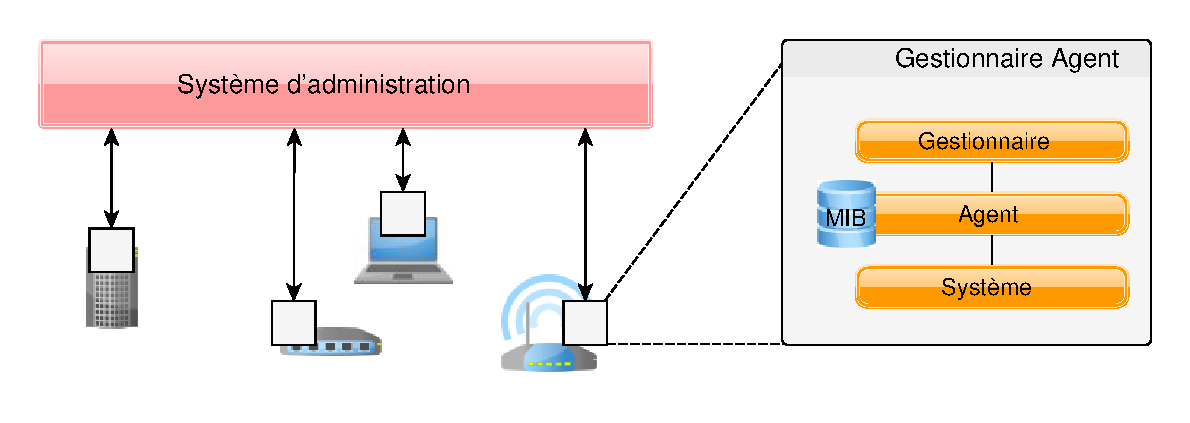
\includegraphics[width=.75\textwidth]{fig/rw-supervision-administration}
    \caption{Architecture d'un système classique d'administration}\label{fig:rw:supervision:administration}
\end{figure}

\subsubsection{Modèles de données}
Il existe plusieurs structures abstraites de données dans le cadre des systèmes d'administrations. La structure la plus répandue reste en l'état la \textbf{structure hiérarchique}. La première apparition d'un tel modèle de donnée remonte à la spécification de SNMP qui prévoit le concept de \textit{Management Information Base} (MIB)~\cite{IETF:MIB}. Une \textit{MIB} est une base d'information où les données sont regroupées sous forme d'arbre. Chaque information possède à l'intérieur de ce arbre un chemin unique (l'\textit{object identifier}) décrit par une suite de chiffres séparés de points. Par exemple, \verb|1.3.6.1.2.1.2.2.1.2| est le chemin décrivant le nom d'une interface réseau sur un dispositif (par exemple \textit{eth0} sur un système Linux). Et le sous-arbre \verb|1.3.6.1.2| (MIB-II~\cite{IETF:MIB-II}) contient toutes les informations concernant les informations réseaux du dispositif.

Par la suite, l'idée des structures hiérarchiques a été reprise pour créer les protocoles d'administrations plus récents comme la structure du modèle des dispositifs de TR-069 (décrit dans le TR-106~\cite{BBF:tr106}) et dans le service de gestion de configuration (CMS) de UPnP-DM~\cite{UPnP:DMCMS}. Dans ces derniers, le modèle de donnée est décrit comme un système de fichier. Les \textit{instances} sont assimilables à des dossiers, et les \textit{feuilles} sont assimilables à des fichiers. Les nœuds ont ainsi un nom et un chemin unique vers la racine \enquote{/}. Tout comme leurs analogues, les \textit{instances} n'ont pas de valeurs associées alors que les \textit{feuilles} contiennent une donnée. Il existe plusieurs types d'\textit{instances} :
\begin{itemize}
    \item \textit{Unique} : Ce nœud peut contenir tout autre nœud. Il représente simplement un chemin intermédiaire un groupe de données.
    \item \textit{Multiple} : Ce nœud peut contenir plusieurs nœuds de type \textit{Instance}. Il permet de représenter une liste de nœuds similaires.
    \item \textit{Instance} : Il représente l'élement de la liste définie par l'instance multiple. Son nom sera toujours un entier pour l'identifier parmi les autres instances. Ces nœuds ont pour vocation à être créés ou supprimés en fonctionnement.
\end{itemize}
\begin{figure}[ht]
    \centering
    \includegraphics[width=.75\textwidth]{fig/rw-supervision-dmtree}
    \caption{Structure hiérarchique du modèle de données d'UPnP-DM}\label{fig:rw:supervision:dmtree}
\end{figure}


Un exemple de modèle de données de ce type de structure est présenté en figure~\ref{fig:rw:supervision:dmtree}. Désormais, une donnée est définie de manière unique, tout comme dans la MIB, grâce à son chemin complet. Dans le vocabulaire du domaine de l'administration, cette donnée est appelé \textit{paramètre}. Le \textit{chemin} d'un paramètre est la concaténation des noms des nœuds qui le sépare de la racine, avec pour séparateur \enquote{/} dans UPnP ou \enquote{.} dans TR-069. Voici quelques exemples de paramètres :
\begin{itemize}
\item \verb|/UPnP/DM/DeviceInfo/PhysicalDevice/HardwareVersion| permet de connaître la version du matériel du dispositif administré. 
\item \verb|/UPnP/DM/Configuration/Network/IPInterface/3/SystemName| est le nom d'une des interfaces réseaux (tout comme \verb|1.3.6.1.2.1.2.2.1.2| dans la MIB). En remplaçant \verb|/3/| par \verb|/5/|, cela concernera une autre interface réseau.
\end{itemize}

L'implémentation de l'agent permettra par la suite de pouvoir créer et remplir cette base d'information.

Toutefois, tous les modèles ne sont pas tous orientés sur la hiérarchie. Il existe notamment l'approche objet adoptée dans les protocoles issues de la DMTF. En effet, dans les protocoles tels que WBEM~\cite{DMTF:WBEM} proposé par le DMTF, la fondation du modèle de données est décrit par un diagramme de classe UML comme présenté en figure~\ref{}.
\begin{figure}[ht]
    \centering
    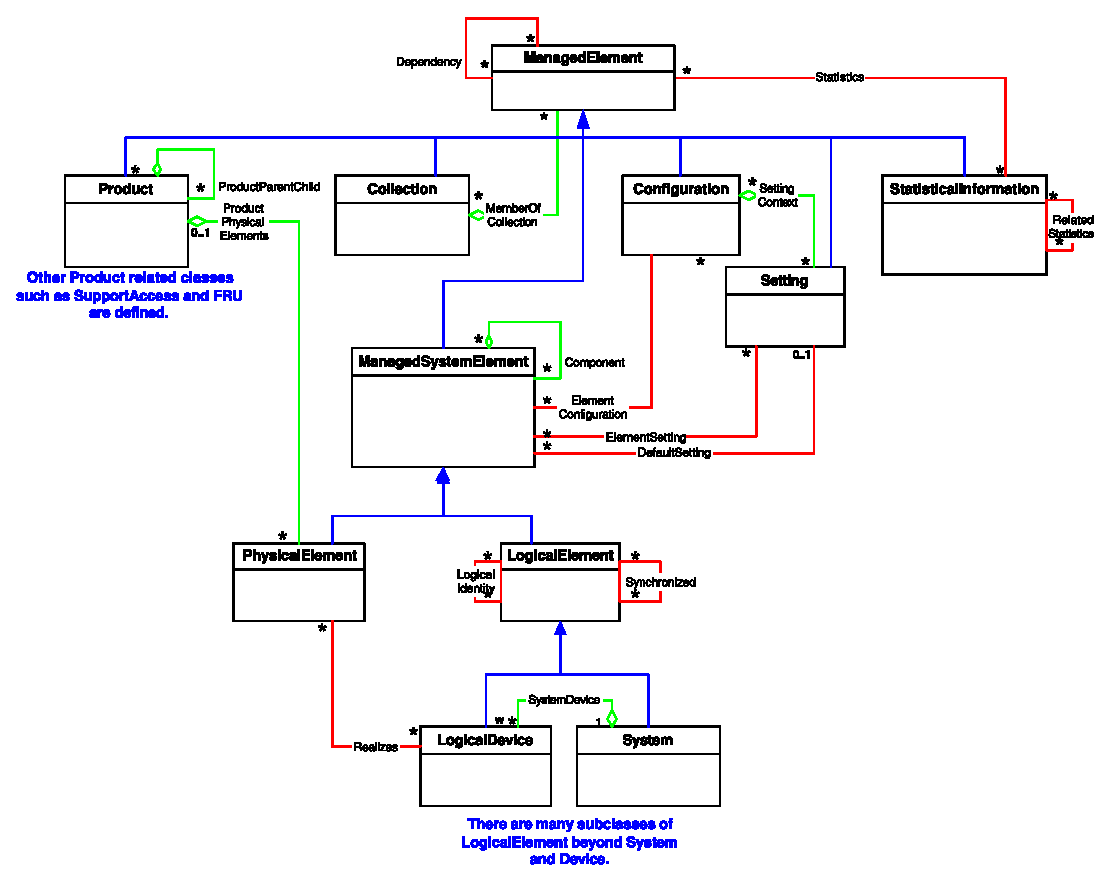
\includegraphics[width=.75\textwidth]{fig/rw-supervision-cimcore}
    \caption{Structure de classe de la partie \textit{Core} de \textit{CIM}}\label{fig:rw:supervision:cimcore}
\end{figure}
\subsubsection{Le gestionnaire global}
Dans l'architecture présentée en figure~\ref{fig:rw:supervision:administration}, 
\subsubsection{Dynamisme des données}
\subsection{Possibles traitements de données}
\subsubsection{L'hétérogénéité par la standardisation}
\subsubsection{Intégration de sources}
\subsubsection{Statistiques}
\subsubsection{Extension du modèle}
\subsection{Synthèse}

\begin{table}[ht]
\criteretabDonnee
    {Principalement structure \textbf{hiérarchique} sous forme de système de fichier. Quelques systèmes d'administration utilisent des modèles objets avec CIM, mais reste difficile à maîtriser.}
    {Une donnée est identifié par son chemin complet. La sémantique est décrite par ce chemin. Pas de contraintes ou inférences exprimées.}
    {Le dynamisme est géré par le mode d'accès. Certains nœuds peuvent être notifiables. D'autres ne sont actualisés que par consultation.}
\criteretabTraitement
    {Instantané et continu sur certaines données. Pas d'hybride possible vu que les procédés sont très séparés.}
    {Standardisation des modèles. Toutes les entités sont structurés dans le même formalisme. Intégration par union des résultats.}
    {Appel de méthodes standardes pour récupérer un sous-arbre du modèle. Code impératif (scripting) pour manipuler les données au niveau du gestionnaire.}
    {Projection simple sur les appels. Certains nœuds particuliers permettent de calculer des statistiques.}
\criteretabAdaptabilite
    {Pas d'adaptation car les dispositifs doivent implémenter des standards.}
    {Pas de perspectives métiers en dehors de la sélection sur les branches du modèle.}
    {Nœuds particuliers pour le calcul. Fonctions métiers intégrées dans le gestionnaire.}
    {Très efficace et utilisé pour gérer des parcs de millions de dispositifs.}
\end{table}
\section{Informatique contextuelle}\label{sec:rw:supervision:contexte}
Au centre des systèmes pervasifs et de l'informatique ubiquitaire, l'informatique contextuelle prend une importance de plus en plus grande. Sa définition a fait l'objet de plusieurs débats au sein de la communauté scientifique. La définition la plus couramment utilisée est : \enquote{L'informatique contextuelle (\textit{context-aware computing} a pour but de permettre aux équipements de fournir de meilleurs services aux utilisateurs par l'utilisation d'informations de contexte}\cite{Han:contextaware}. Ainsi, le point important est de former un ensemble d'information pour que des applications puissent adapter leur fonctionnement. L'instanciation de cette notion de contexte est un processus d'observation de l'environnement dans lequel se trouve l'application.

La section~\ref{sec:rw:supervision:administration} a permis de voir que le système observé peut fournir de grandes quantités de données. Grâce à l'informatique contextuelle, nous souhaitons pouvoir donner de la cohérence à ces données. Ainsi, nous pouvons mieux exploiter leur sémantique et envisager d'effectuer de l'observation de plus haut niveau afin d'établir un diagnostic.

Cette section présente d'abord les définitions et applications de l'informatique contextuelle. Par la suite, nous détaillons la façon dont le contexte est capturé et modélisé. Nous présentons les capacités de traitement sur celui-ci. Enfin, nous analysons différents systèmes pervasifs afin de percevoir la mise en application de cette approche. Nous concluons par une synthèse, détaillant l'adéquation aux critères de notre problématique.

\subsection{Définitions et applications}
La définition de contexte a été elle aussi au cœur de nombreux débats. Après analyse des travaux sur le sujet, le rapport de recherche~\cite{Dey:context} propose la définition suivante : \enquote{\it Un contexte est toute information pouvant être utilisée pour caractériser la situation d'une entité. Cette entité pouvant être une personne, un lieu, ou un objet considéré comme pertinent à l'interaction entre l'utilisateur et le système.}.

Il est important de noter que cette définition est orientée par l'utilisation qui en est faite. Une donnée quelconque peut faire partie d'un contexte si elle est utilisée comme tel. Ainsi, il est nécessaire de voir l'ensemble des utilisations de ce contexte. Celles-ci sont rassemblées dans sept catégories principales~\cite{Soylu:context} : 
\begin{enumerate}
	\item Sélection et recommandations d'informations ou de services.
	\item Présentation et accès à l'information et aux services.
	\item Recherche d'information ou de service.
	\item Adaptation de l'exécution de processus séquentiels.
	\item Modification et reconfiguration d'applications.
	\item Conseil d'actions semi-automatique.
	\item Allocations de ressources.
\end{enumerate}
Les utilisations du contexte sont directement reliées à l'observation, car c'est elle qui permet la construction du contexte.

\subsection{Modélisation et capture du contexte}
Le modèle utilisé pour créer et manipuler le contexte peut être de différentes formes : basé sur des principes d'intelligence artificielle (représentations de connaissances, réseaux bayésiens), le génie logiciel (UML), les bases de données (ER : Entité-Relation) ou d'autres moyens applicatifs (arbres, entrées clefs-valeurs). L'UML et l'ER atteignent rapidement leurs limites d'expressivité. Il devient difficile de manipuler les données dans le cadre de contextes larges et hétérogènes à cause de leur rigidité. Ces modèles permettent d'abstraire une partie du monde ou de la logique pour un usage restreint. Par opposition, la gestion de données issues d'ontologies est moins soumise à cette rigidité.

\subsubsection{Un modèle sous forme de triplet}
Pour représenter l'ensemble des connaissances sur le système, autant en terme de structure que de données, les contextes sont la plupart du temps modélisés comme un réseau sémantique. Le langage communément utilisé pour cela est le RDF (\textit{Resource Description Framework})~\cite{W3C:RDF}, un standard répandu. Son principe est à la fois simple et puissant. Son expression est simple, car toute sa structure est orchestrée par des triplets : Objet, Relation, Valeur. Par exemple, \textit{la télévision} \textbf{est située dans} \textit{le salon}. De même, \textit{le salon} \textbf{est une} \textit{pièce}. L'ensemble des triplets forme un graphe où les objets et valeurs sont des nœuds et les relations sont des liens, d'où l'appellation de \textit{graphe sémantique}~\cite{Minsky:knowledge}. Pour étendre l'expressivité des graphes sémantiques et y apporter la notion de classes, les ontologies se sont développées.

\subsubsection{Les ontologies}
Tel que l'a défini Kalfoglou~\cite{Kalfoglou:ontology}, une ontologie est \textit{une représentation explicite d'une compréhension commune de concepts importants appartenant à un domaine d'intérêt}.
Elle permet de capturer et de représenter une vue simplifiée d'un domaine à travers des concepts prédéfinis. Cela permet un langage commun et une taxonomie des concepts, mais aussi, l'ontologie est capable de représenter leurs liaisons. Ainsi, il est possible de modéliser la sémantique propre des différentes données.

Les ontologies sont toutefois structurées dans un langage qui permet de définir les grandes catégories de relations ou d'objets. Plusieurs langages existent, mais tous définissent les entités suivantes :
\begin{itemize}
    \item[\textbf{Concepts}] Décrivent les classes et sous-classes de toutes les choses du monde.
    \item[\textbf{Instances}] Ce sont les individus correspondant aux concepts.
    \item[\textbf{Relations}] Permet de lier les concepts et instances entre eux. Une des relations principales est la relation \textit{Est-Un} (\textit{Is-A} en anglais) qui lie une instance à un concept.
    \item[\textbf{Types de données}] Types syntaxique d'une donnée : entier, chaîne de caractères, booléen.
    \item[\textbf{Valeurs}] Valeur qu'un concept ou instance peut avoir.
\end{itemize}

Par la suite, les langages permettent différentes manières de lier les concepts entre eux. Cette capacité va permettre de montrer l'expressivité de la structure. Par exemple, une des relations des plus importantes est la relation de hiérarchie. Un \textit{chien} \underline{est une sous-classe d}'\textit{animal}, et \textit{labrador} \underline{est une sous-classe de} \textit{chien}. La \textit{relation de hiérarchie} \underline{est une} \textit{relation transitive}. Ainsi, le langage vérifie naturellement que le \textit{labrador} \underline{est une sous-classe d}'\textit{animal}. 

La logique permettant d'exprimer ces contraintes et inférences structurelles est une logique de description. Suivant la classe de la logique de description sous-jacente, le langage est plus ou moins complexe à traiter par la suite\footnote{Dans certains cas, comme OWL-Full, son expressivité est tellement large qu'il devient indécidable de vérifier si un concept appartient à une classe.}. Par exemple, le langage le plus utilisé reste \textit{OWL Lite}, équivalent à la logique $\mathcal{SHIF}^\mathcal{(D)}$. Cette logique permet lors de la description des concepts l'utilisation des constructeurs suivants : quantification universelle, négation\footnote{Si la négation et la quantification universelle existent, alors le prédicat d'existence est autorisé, car $\not\forall \equiv \exists$}, transitivité de relation, inversion de relation, hiérarchie de relations. De plus, l'usage de propriétés fonctionnelles et de données est possible. En revanche, la restriction d'une collection à un nombre d'éléments donné par exemple n'est pas possible. Son utilisation est répandue, car les inférences sont calculables dans la pratique contrairement à des logiques plus expressives.

Comparées à des structures telles qu'UML, les ontologies jouissent de la flexibilité des réseaux sémantiques. Il est toutefois important de noter que cette puissance et cette liberté rendent sa manipulation délicate. En effet, il est supposé que toutes les sources de connaissances s'appuient sur une ontologie commune. Il est important d'être minutieux dans la manipulation de cette structure pour éviter par exemple des duplications de concepts, voire des conflits de définitions.

\subsubsection{Capture du contexte}
La capture du contexte est la manière de récupérer une information et de la représenter sous la forme choisie lors de la modélisation. Par exemple, un capteur de température peut insérer un ensemble de triplets pour indiquer qu'à 10h25 le lundi 26 avril, il faisait 25.256ºC sur la source T75896. Cet ensemble de triplets dépend de la modélisation des concepts qui forme le contexte. Lors de la capture, les données sont issues du système observé ou par l'extraction de nouvelles connaissances construites à partir d'informations déjà capturées.

La gestion de l'hétérogénéité est rarement mentionnée puisque les sources de données sont censées être conformes au schéma commun. Toutefois, comme présenté dans~\cite{Kaed:these}, il est possible d'aligner les modèles des sources avec un schéma commun. Le formalisme des ontologies permet en effet de décrire les équivalences logiques entre différents concepts ce qui permet l'intégration de données.

\subsection{Capacités de traitement}
Un intérêt des réseaux sémantiques est le pouvoir de raisonnement logique. Le but ici est de pouvoir inférer de nouveaux triplets à partir des connaissances accumulées. Pour cela, il existe plusieurs langages permettant de spécifier ces inférences. Le plus courant est le langage associé à \textit{RDF} : \textit{SPARQL}. Ce langage a la particularité d'être aussi expressif que l'algèbre relationnelle~\cite{Angles:sparql}\footnote{Plus exactement, SparQL est équivalent au \textit{datalog} non récursif avec négation, ce qui est équivalent à l'algèbre relationnelle.}. Ainsi, il est possible de faire des inférences du premier ordre sur ces données.

Ces inférences sont de trois types :
\begin{itemize}
 \item[\textbf{Association directe}] Une information bas-niveau est associée à une information haut-niveau 
 \item[\textbf{Fusion de contexte}] Un ensemble de données infère un nouvel état 
 \item[\textbf{Fission de contexte}] Une donnée infère un ensemble d'informations
\end{itemize}

Dans l'informatique contextuelle, il est important de distinguer plusieurs espaces de données~\cite{Padovitz:agent} :
\begin{itemize}
 \item[\textbf{L'espace de valeur}] Par exemple, pour une personne, son age est compris entre 0 et 125.
 \item[\textbf{L'espace applicatif}] L'ensemble des données atomiques qui représentent le contexte dit de bas-niveau.
 \item[\textbf{L'espace de situation}] Reflète les situations pouvant être extraites de l'espace applicatif.
\end{itemize}

À un instant donné, il est possible de définir un \textbf{état de contexte} en tant que collection d'attributs de l'espace de contexte. Cet état peut par la suite inférer un ensemble de situations. La figure~\ref{rw-supervision-contextreasoning} résume la structure abstraite du raisonnement sur les contextes.

\begin{figure}[ht]
    \centering
    \includegraphics[width=.50\textwidth]{rw-supervision-contextreasoning}
    \caption{Structure abstraite du raisonnement sur contexte. À un élément du contexte $c_i$ est associée une valeur du domaine $V_i$. À partir de l'espace du contexte $C$, on effectue des associations, des fissions ou fusions pour inférer l'espace des situations $S$.}\label{rw-supervision-contextreasoning}
\end{figure}

\subsubsection{La qualité de contexte}
La qualité du contexte~\cite{Buchholz:quality} est définie comme toute information permettant de décrire la qualité des informations contenues dans le contexte. Le point crucial est que cette qualité n'est pas liée à un quelconque processus ou matériel. Elle peut se décliner en plusieurs \textit{paramètres} : précision, fiabilité, confiance, fraicheur,\dots{}

La qualité des données a des impacts lors du diagnostic. Supposons que nous constatons un problème de pixélisation TV. Cette situation a été inférée par la valeur actuelle d'une métrique indiquant le nombre d'images non décodées. Premièrement, si la source de donnée remontant la métrique n'est pas assez fiable, nous pouvons mettre en doute les relevés. De plus, il est possible que l'information ne reflète pas l'état actuel. Ainsi, la situation indiquant un problème est vraie à la qualité des sources près.

De plus, si nous souhaitons effectuer un diagnostic, nous pouvons indiquer au système que ce type de panne est dû à un problème de lenteur de réseau interne. Toutefois, ce peut être dû à des dysfonctionnements plus rares, comme une panne matérielle. Ainsi, certaines recherches permettent d'introduire une part de probabilités dans les raisonnements pourtant déterministes a priori~\cite{Padovitz:agent}.

Dans cette thèse, nous ne détaillons pas le concept de qualité des données. Néanmoins, nous pouvons voir que cela peut avoir des impacts majeurs. L'utilisation de ces travaux serait intéressant pour des améliorations futures.

\subsection{Analyse de systèmes d'observation à base de contextes existants}
Dans cette partie, nous analysons des systèmes pervasifs à base de contexte existant. Ceux-ci sont en général très utilisés dans le réseau domestique qui est l'environnement de développement le plus courant dans le domaine de l'informatique ubiquitaire. Cette étude nous permet de voir comment est mise en pratique l'approche présentée jusqu'ici.

\subsubsection{De la représentation du système}
\textit{DogOnt}~\cite{Bonino:dogont}, a pour objectif de pouvoir modéliser les objets des environnements domotiques intelligents. Ainsi, en plongeant l'ensemble des équipements au niveau conceptuel des ontologies, il est possible de résoudre les problèmes d'interopérabilité et d'hétérogénéité des données. \textit{DogOnt} est capable de répondre à des requêtes telles que : la position de l'équipement, ses capacités, ses moyens de communication, comment l'environnement est composé (notamment architecturalement parlant, ce qui permet de représenter la maison).

Ainsi, une représentation de haut niveau permet de poser tous les concepts afin de représenter le réseau domestique au sens large. D'une manière plus concrète, un équipement est représenté en tant que \enquote{\it Controllable} (et ses sous-classes). Cette ontologie est représentée dans la figure~\ref{fig:rw:supervision:dogont}.

\begin{figure}[ht]
    \centering
    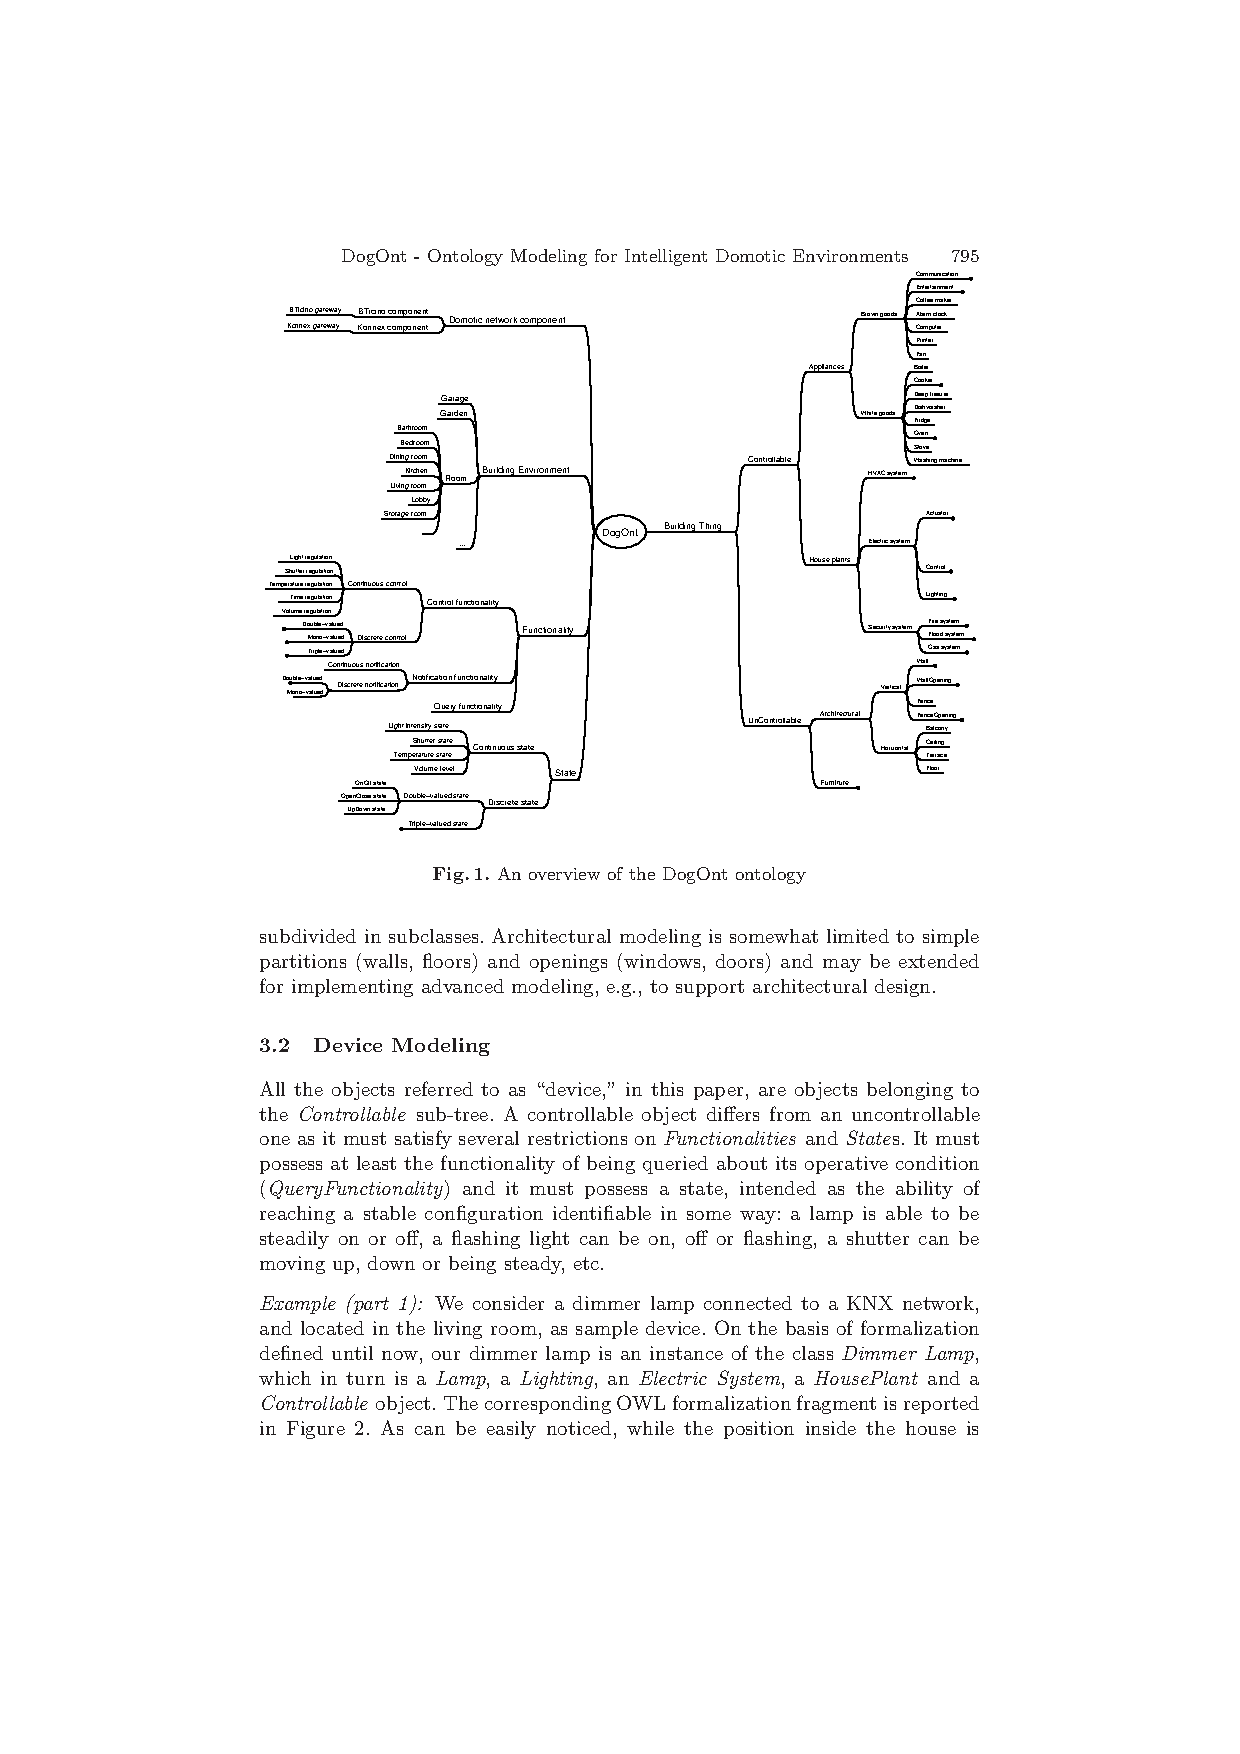
\includegraphics[width=0.8\textwidth, trim=4cm 15.5cm 4cm 4.6cm, clip]{rw-supervision-dogont}
    \caption{L'ontologie de DogOnt}\label{fig:rw:supervision:dogont}
\end{figure}
Pour pouvoir observer, et contrôler, les instances de ces concepts, il est nécessaire de rajouter des fonctionnalités et des variables d'états. Ceci se fait par l'introduction de relations sémantiques telles que \textit{hasControl}, \textit{hasFunctionality}, et \textit{hasState}. En combinant ces associations ainsi que l'ensemble complet des instances, il est possible de représenter l'ensemble des périphériques et leurs capacités.

Plusieurs autres projets ont utilisé ce type de modélisation pour des applications pervasives. Par exemple, Amigo~\cite{BenMokhtar:easy} se focalise plus sur la modélisation des services et des capacités. A contrario, \textit{MATCH}~\cite{Docherty:match} met l'accent sur la hiérarchie des ontologies pour que chaque domaine puisse apporter ses connaissances en utilisant des concepts communs (\textit{dispositifs}, \textit{réseau},\dots).

Nous remarquons que la séparation des domaines permet de gérer les perspectives utilisateurs en fonction de leurs intérêts. De plus, nous notons que l'hétérogénéité des schémas conceptuels est gérée par l'utilisation d'une ontologie commune. La nécessité d'une ontologie commune est récurrente dans ces travaux. Toutefois, dans des travaux récents~\cite{Niang:global,Niang:integration}, il existe des approches semi-automatiques pour intégrer des données de sources hétérogènes via la génération d'une ontologie commune et d'alignements.

\subsubsection{SOCAM : De l'utilité du raisonnement logique}
SOCAM (Service-Oriented Context-Aware Middleware)~\cite{Gu:socam} propose un intergiciel générique pour permettre aux développeurs de créer des applications pervasives par contexte. Cet intergiciel supporte l'acquisition, la découverte, l'interprétation et l'accès aux contextes. Comme les autres solutions présentées jusqu'ici, il s'appuie sur une ontologie conceptualisée comme celle de \textit{MATCH} afin de pouvoir être générique et y apporter les connaissances de chacun des domaines.

L'architecture de SOCAM, représentée en figure~\ref{fig:rw:supervision:socam} qui se décrit en trois 4 composants principaux.
\begin{figure}[ht]
    \centering
    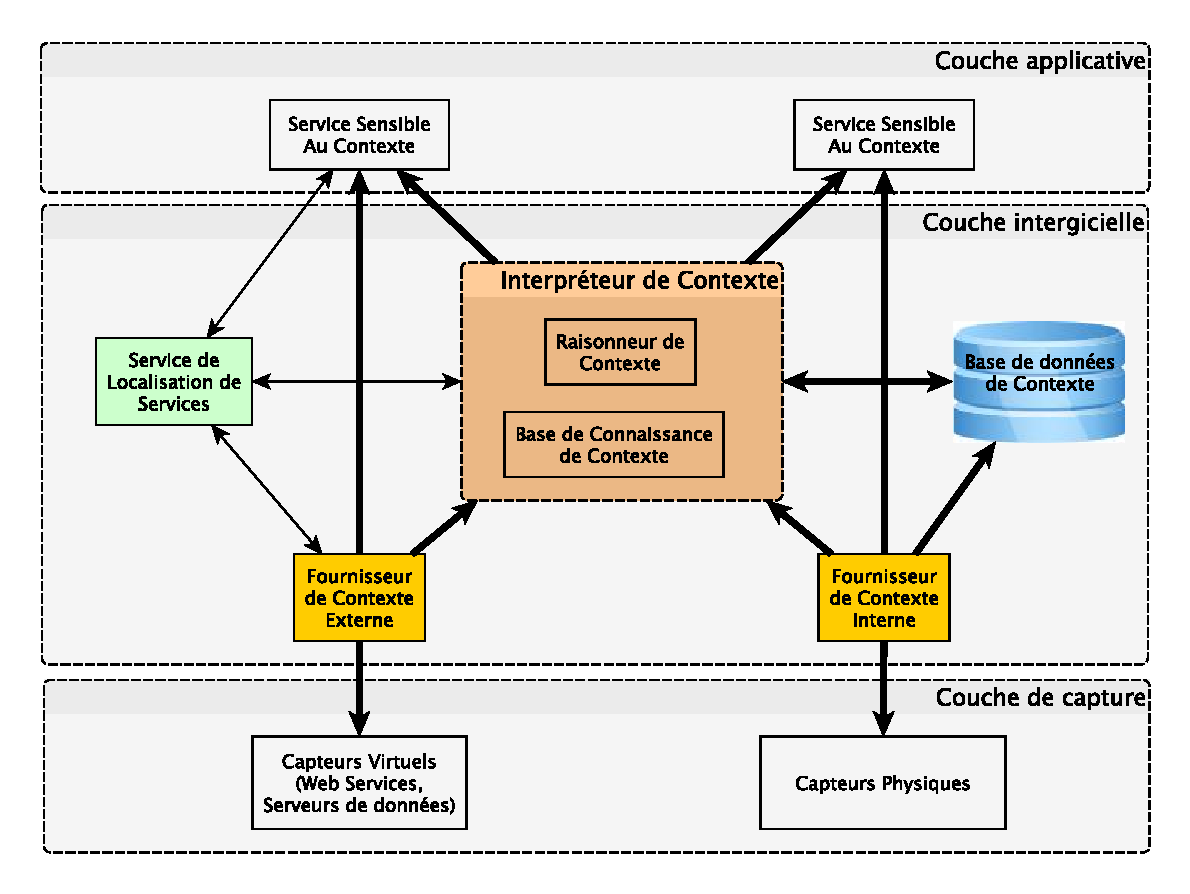
\includegraphics[width=0.66\textwidth]{rw-supervision-socam}
    \caption{Architecture de SOCAM}\label{fig:rw:supervision:socam}
\end{figure}
\begin{itemize}
	\item[\textbf{Fournisseurs de contexte}] Qui permet d'abstraire l'hétérogénéité des données issues des différentes sources (internes, tels que les capteurs ou autres dispositifs), ou externe (services météo ou autres) pour les convertir en \textit{OWL}.
    \item[\textbf{Interpréteur de contexte}] Fournit la logique de raisonnement sur le contexte.
    \item[\textbf{Base de données de contexte}] Stocke les ontologies de contexte et l'historique des contextes pour chaque sous-domaine.
    \item[\textbf{Service de localisation de services}] Sert de catalogue des services externes disponibles. Sa sélection peut se faire sur un type de service, mais il peut aussi faire une comparaison sur le contexte que le service fournit.
\end{itemize}
Les services applicatifs utilisant la notion de contexte vont ainsi utiliser les fonctionnalités que fournit SOCAM pour gérer cet ensemble de données. Une manière classique de construire ces services est de spécifier des actions déclenchées par un ensemble de règles au moment où le contexte change.

SOCAM implémente deux manières de faire de l'inférence logique de prédicats. La première est l'inférence structurelle. En effet, l'application d'une propriété transitive à un concept nous donne plusieurs informations. Par exemple, nous pouvons inférer que l'appareil \textit{Livebox} est une passerelle internet. Or, tous les équipements de cette catégorie ont des propriétés telles que la capabilité à gérer les règles de routage. La deuxième manière d'inférer des informations est un ensemble de règles utilisateurs. En utilisant un moteur similaire aux moteurs \textit{Prolog}, il est possible d'induire des informations qui constituent l'ensemble des situations. Par exemple, les auteurs présentent l'inférence du triplet \textit{(user socam:status 'SLEEPING')} par la détection de la position allongée dans la chambre avec la lumière éteinte.

Nous remarquons ici la présence d'une couche de traitement de données entre les sources et les services qui les utilisent. Cette couche se base sur des inférences logiques qui utilisent un support persistant pour constituer son contexte.

\subsection{Synthèse}
En conclusion, le traitement contextuel des données permet de gérer l'hétérogénéité sémantique des données. Les capacités de traitements sont liées à l'inférence logique pour enrichir la base des connaissances accumulées. Ainsi, il est possible de construire un espace de contexte et d'en inférer des situations de haut niveau. Cette capacité d'abstraction est nécessaire pour l'informatique ubiquitaire qui a besoin de manipuler des concepts humains.

Pour notre problématique d'observation, il reste difficile de gérer l'évolution des données au cours du temps. La liberté d'expression des bases de connaissances fait que l'inférence est complexe à manipuler. Plusieurs travaux s'attellent à permettre aux connaissances et aux règles d'introduire la dimension dynamique~\cite{Weikum:webknowledge, Hellerstein:declarative}. L'apport de cette dimension est toutefois difficile d'un point de vue théorique.

\begin{table}[!ht]
\criteretabDonnee
    {Structure sémantique à base de triplet.}
    {Utilisation d'ontologies. Gestion des contraintes et de l'inférence structurelles variable suivant l'expressivité du langage. En général, \textit{OWL Lite} est utilisé.}
    {Pas de gestion explicite du dynamisme en dehors d'annotations.}
\criteretabTraitement
    {Instantané uniquement.}
    {Les sources s'intègrent en se conformant à un modèle commun. Si tel n'est pas le cas de façon native, des règles d'alignements d'ontologies sont à fournir.}
    {Paradigme déclaratif en général dérivé de programmation logique allant de \textit{Prolog} à \textit{SPARQL}.}
    {Cela part de la logique du premier ordre complète à la capacité de l'algèbre relationnelle (\textit{datalog} non récursif avec négation)}
\criteretabAdaptabilite
    {Nécessité de spécifier des ontologies de domaines pour donner la structure des concepts du système.}
    {La séparation des domaines et le rattachement des données aux domaines permettent de clairement spécifier les différentes perspectives.}
    {Pas d'extensibilité possible sur le traitement d'inférence. Par contre, il est possible suivant l'architecture du système final de créer des capteurs de contextes pour fournir des données logiques de haut niveau.}
    {La complexité de l'inférence peut aller jusqu'en \textit{EXPTIME}. Toutefois, plusieurs implémentations optimisées permettent de traiter des millions de triplets en quelques secondes.}
\caption{Synthèse de l'informatique contextuelle}\label{tab:rw:supervision:contexte:synthese}
\end{table}

\section{Entrepôts de données}
asdwd
\section{Gestion de flux de données}
Devant la multiplication des applications à base de flux de données telles que : la gestion des données de capteurs ou la surveillance réseau, les systèmes de gestions de flux de données (\textit{SGFD}) ont étés conçus. L'idée principale de ce type de système étant de permettre une utilisation des flux de données de la même manière que les bases de données. L'interrogation des flux passerait donc par un langage déclaratif (tout comme le \textit{SQL}) avec un grand pouvoir d'expression.
\subsection{Approche des SGFD}
Un flux de données est une série de données qui s'accumule au fur et à mesure du temps. De façon général, il n'est pas supposé une régularité temporelle sur l'arrivée des données dans le flux (tel que \enquote{\it une donnée toutes les 5 secondes}). L'idée de faire une interrogation sur ces flux de données au sens \enquote{gestion de base de données} du terme n'a pas de sens car il y aurait confusion entre les modes d'interrogations continues et instantanées présentés en section~\ref{sec:rw:supervision:criteres:traitement}. En effet, le paradigme des requêtes est fondamentalement différent~\cite{Gurgen:sstreamware}.
\begin{figure}[ht]
    \centering
    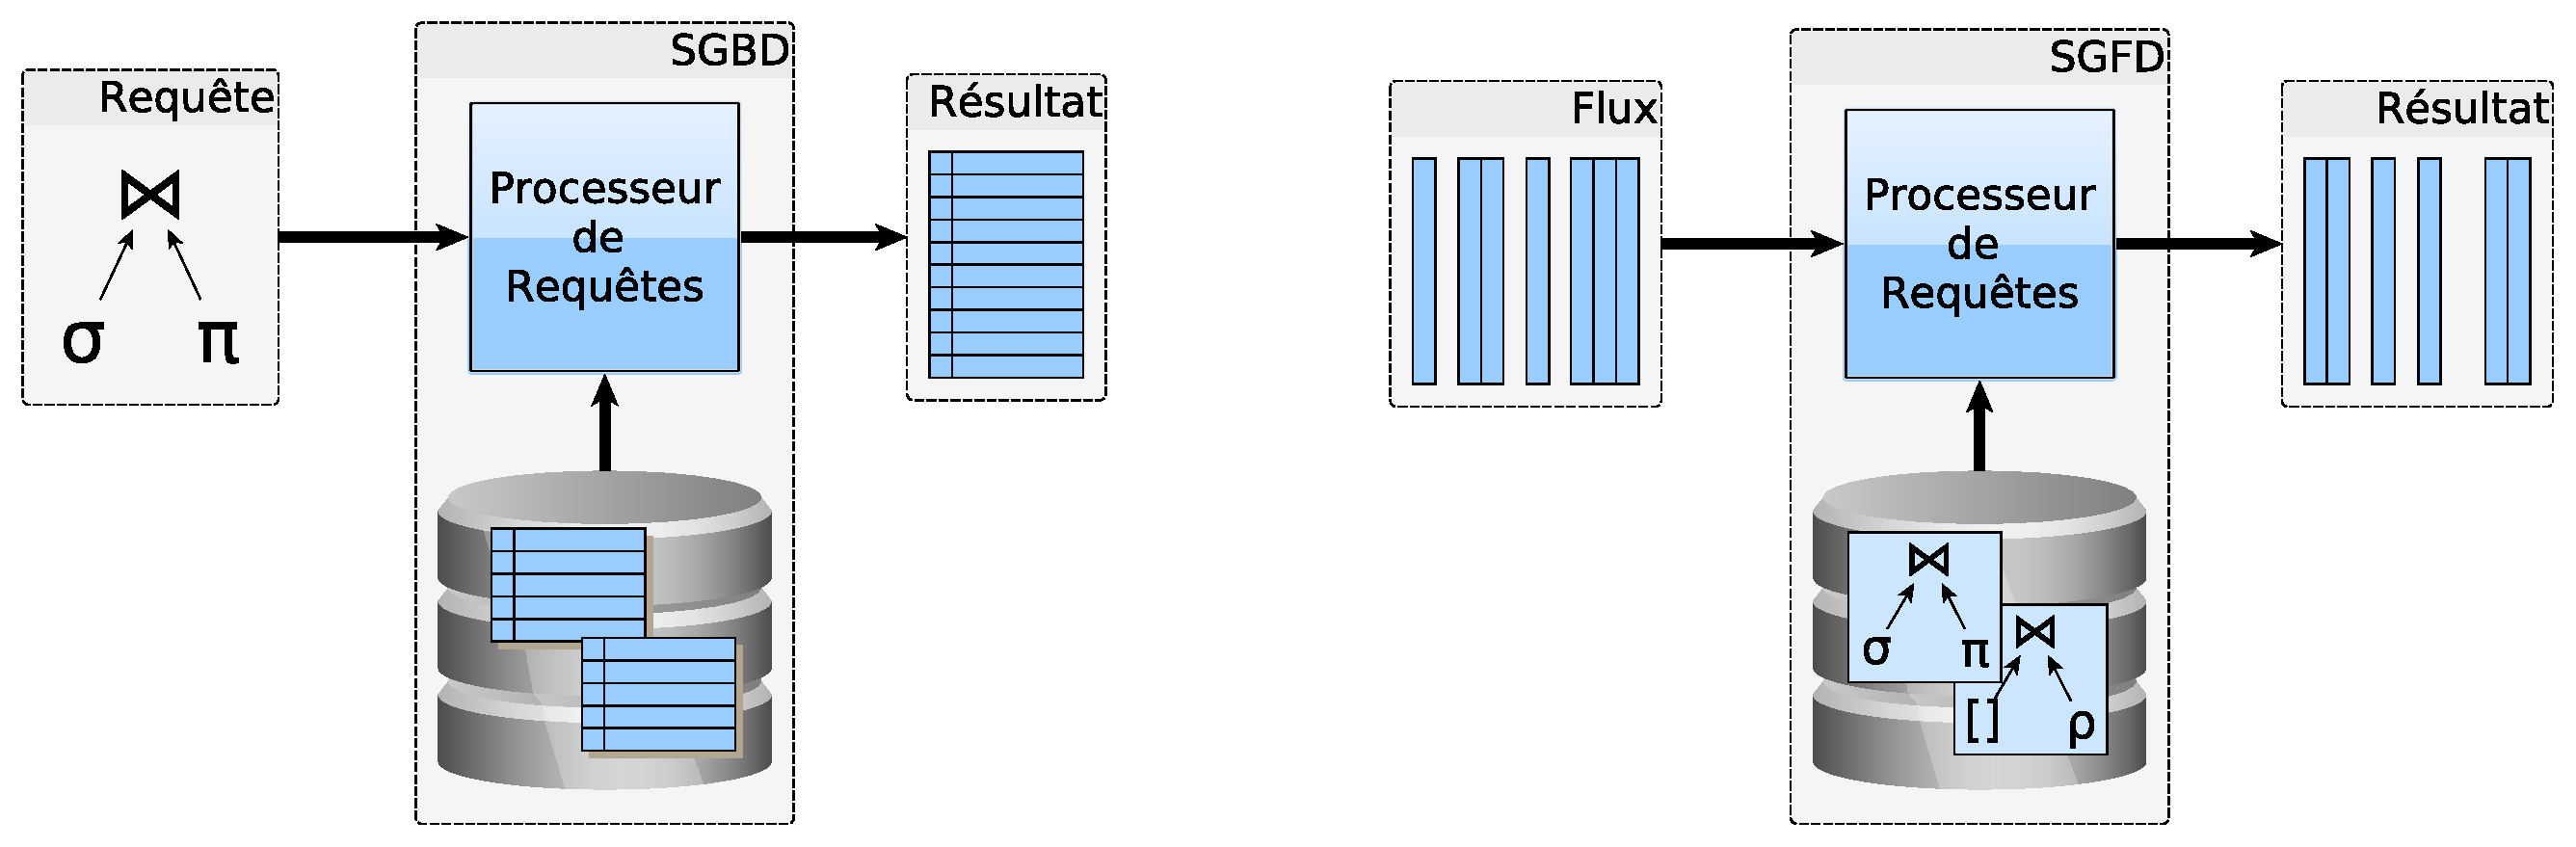
\includegraphics[width=0.75\textwidth]{rw-supervision-sgbd-sgfd}
    \caption{SGBD : Requêtes transitoires, Données persistantes vs SGFD : Données transitoires, Requêtes persistantes}
\end{figure}

\begin{itemize}
    \item[\textbf{Base de données}] : Une requête est une question posée sur un ensemble de relations figées et persistants (principe transactionnel). La réponse est un ensemble de n-uplets. Une fois la requête traitée elle n'existe plus.
    \item[\textbf{Flux de données}] : Une requête un ensemble d'opérateurs et est considéré comme persistant. Le ou les flux de données sont appliqués sur cet ensemble d'opérateurs pour en produire un nouveau flux.
\end{itemize}

\subsection{Principes architecturaux}
\subsection{Les opérateurs}
\subsection{Synthèse}
\begin{table}[!ht]
\criteretabDonnee
    {Modèle dérivé du relationnel mais où le contenu est variable dans le temps.}
    {Pas de structure sémantique en dehors de gestion de méta-données.}
    {Toutes les données sont dynamiques et événementielles a priori.}
\criteretabTraitement
    {Continue.}
    {Il est supposé que chaque source produit un flux de données. Le fait de traiter ces flux participe à l'intégration de sources.}
    {Langages de requêtes similaires aux SQL supportant la dynamique et l'évolution des données}
    {A un instant donné, les opérateurs sont semblables au relationnel. L'expressivité du support du dynamisme reste inconnu encore.}
\criteretabAdaptabilite
    {Création de source pour fournir les flux de données. Comme il n'y a pas de structure sémantique, l'adaptation n'est que l'écriture de requêtes continues.}
    {Pas de perspectives métiers.}
    {Les sources et puits sont en général adaptés par les utilisateurs. Un développement peut être fait dessus, mais il est rarement possible de rajouter des opérateurs.}
    {Très rapide car la latence de traitement doit être contrôlée pour supporter des haut débits.}
\caption{Synthèse des systèmes de gestion de flux de données}\label{tab:rw:supervision:sgfd:synthese}
\end{table}

\section{Conclusion}
Après 20 années de recherche, la gestion de flux de données devient désormais suffisamment mature pour être appliqué massivement. Plusieurs produits commerciaux sont d'ailleurs maintenant utilisés en production. Toutefois, nous pouvons nous rendre compte que la complexité théorique de ces systèmes a été sous-estimé. De nombreux modèles ont été décrit pour représenter les flux de données et leurs traitements. Ces modèles sont encore remis en questions aujourd'hui au fur et à mesure des applications concrètes. 

Nous avons vu que le problème d'avoir une bonne connaissance du modèle et du comportement théorique des SGFD est crucial. En l'état, l'intégration des supports persistants reste ad-hoc et assisté par l'utilisateur. Un fonctionnement intégré avec une modélisation générique capable de gérer les deux modes d'interrogations de façon unifiée est donc indispensable pour manipuler correctement flux et relations persistantes. Similairement, les contributions sur l'optimisation de traitement des requêtes sont encore principalement ponctuelles. Afin d'appliquer un traitement efficace pour toute requête, il est nécessaire d'avoir une bonne connaissance théorique du traitement.

Notre contribution technique se concentrera sur trois points principaux :
\begin{itemize}
 \item[\textbf{Modélisation}] : Création d'Astral, algèbre de traitement des requêtes continues sur flux et relations temporelles. Nous accorderons de l'importance sur la prise en compte des problèmes relevés en section~\ref{sec:rw:sgfd:modeles:synthese}. Cette algèbre sera présenté dans le chapitre~\ref{chap:contrib:astral}
 \item[\textbf{Exécution}] : Mise en œuvre de l'intergiciel Astronef pour construire et exécuter efficacement une requête exprimée avec l'algèbre Astral. Ainsi, à partir d'une requête algébrique, il est possible de sélectionner le plan de requête qui semble le plus efficace grâce aux connaissances accumulés. Cette mise en œuvre sera développée dans le chapitre~\ref{chap:contrib:execution}.
 \item[\textbf{Persistance}] : Conception de l'extension Asteroid permettant l'intégration des requêtes continues sur flux et des requêtes sur support relationnel persistant. Ceci permettra de gérer la représentation du système observé ainsi que l'historisation des données dynamiques. Le support mathématique de cette intégration sera supporté par Astral et sa mise en œuvre par Astronef. Cette intégration sera effectuée dans le chapitre~\ref{chap:contrib:persistance}.
\end{itemize}

Grâce à ces contributions, il deviendra possible de mettre en œuvre un système d'observation générique applicable sur tout type de données. L'utilisateur devra exprimer des requêtes dans le langage algébrique Astral. Une fois ces requêtes écrites, nous serons garanti de leur mise en œuvre. Le tableau~\ref{tab:rw:contrib} résume l'ensemble des points d'analyses que nous nous étions fixés en section~\ref{sec:rw:supervision:criteres}.
\begin{table}[!ht]
\criteretabDonnee
    {Relationnel dérivé. Nous réutilisons les principes utilisés dans la gestion de flux et des bases de données.}
    {\good Modèle entité-relation augmenté pour supporter les flux.}
    {\good Requêtes sur tout type de données (flux, relations).}
\criteretabTraitement
    {\good Continue, Instantannée, Mixte}
    {\good Utilisation des requêtes continues des SGFD en tant qu'intégrateur.}
    {\meh Astral : langage de requête algébrique. Un langage purement déclaratif reste toutefois dérivable de ces fondations théoriques.}
    {\good Relationnel avec support \textbf{intégré} du dynamisme des données.}
\criteretabAdaptabilite
    {\good Spécification du modèle du système ainsi que des requêtes d'intégration (algébriques).}
    {\meh Pour l'analyse, la gestion de données multi-dimensionnelles des entrepôts utilisés est utilisé. Pour l'interrogation continue, utilisation d'un opérateur de préférences sur les flux.}
    {\good Infrastructure générique capable de supporter l'ajout d'opérateurs avec plusieurs implémentations.}
    {\good Héritage de l'efficacité des flux de données. Sélection du meilleur plan d'exécution pour chaque requête. Héritage des supports de grands volumes grâce aux entrepôts.}
\caption{Résumé de notre contribution selon nos critères}\label{tab:rw:contrib}
\end{table}

\begin{savequote}[6cm]
\enquote{
    Now that I know what they all do 

    I have to find my place 

    And help with all of my heart 

    Tough task ahead I face
}
\qauthor{Twilight Sparkle, Winter Wrap Up}
\end{savequote}

\chapter{Systèmes de Gestion de Flux de Données}\label{chap:rw:sgfd}
\chaptertoc
Nous avons présenté dans le chapitre précédent les concepts de la gestion de flux de données. Celle-ci permet de répondre à l'interrogation continue des données temps réel. Dans ce chapitre, nous explorons ce domaine d'un point de vue plus technique afin d'identifier nos points de contributions pour exploiter ce domaine pour l'observation de systèmes.

Ce chapitre est organisé en quatre sections. Tout d'abord, la section~\ref{sec:rw:sgfd:modeles} présente les formalisations théoriques analyser les capacités d'interrogation des SGFD. Par la suite, nous présentons les infrastructures de traitement en section~\ref{sec:rw:sgfd:infra}. Cette section analyse l'impact des modèles théoriques et les limitations de leur mise en œuvre. Ainsi, il devient possible d'analyser l'intégration des supports persistants aux infrastructures de traitements en section~\ref{sec:rw:sgfd:persistance}. Enfin, nous observons des aspects liées aux performances en présentant les recherches sur les optimisations en section~\ref{sec:rw:sgfd:optim}. Nous concluons en présentant une synthèse et une description des points techniques de contributions sur lesquelles nous intervenons dans les chapitres suivants.

\section{Modèles théoriques}\label{sec:rw:sgfd:modeles}
Nous avons présenté brièvement dans le chapitre~\ref{chap:rw:supervision} que les systèmes de gestions de flux de données s'inspiraient du modèle relationnel. Le modèle relationnel ne supporte toutefois pas le dynamisme des données. Ainsi de nombreuses propositions ont été faites dans l'état de l'art pour reconstruire un modèle tout en tentant de réutiliser les connaissances développées sur les systèmes de gestion de base de données relationnels depuis 40 ans.

Dans cette section, nous allons détailler l'historique de la recherche dans ce domaine. Pouvoir observer l'évolution des modèles au fur et à mesure des années permet en effet de bien cerner les problématiques théoriques lié à la gestion de flux. En~\ref{sec:rw:sgfd:modeles:early}, nous présenterons l'établissement des premiers modèles. En~\ref{sec:rw:sgfd:modeles:stream}, nous présenterons la sémantique abstraite mélangeant flux et relations. Puis nous présenterons en~\ref{sec:rw:sgfd:modeles:batch} les initiatives de clarifications et reformalisation des modèles existants. Enfin, nous présenterons une synthèse de ces travaux.

\subsection{La genèse de la gestion de flux}\label{sec:rw:sgfd:modeles:early}
L'idée de créer des requêtes continues a été présenté en 1992 dans le système Tapestry~\cite{Terry:tapestry}. Dans ce système une requête continue est avant tout une requête instantanée, mais la sémantique étant que celle-ci sera exécuté périodiquement. Ces requêtes s'appliquent sur un ensemble de données sans suppression ou mise à jour (\textit{append-only}). Le résultat de cette requête sera représenté par le flux des nouvelles données calculés de manière incrémental. Pour cela, les relations sont réellement considérés comme des variables et elles deviennent donc dépendantes du temps.

En 1995, les flux de données ont été explorés tout d'abord par le modèle séquentiel $\mathcal{SEQ}$~\cite{Seshadri:seq}. Dans ce modèle, une \enquote{\it séquence} est un ensemble d'enregistrements (n-uplets relationnels) avec un ordre positionnel. Dans le modèle relationnel originel~\cite{Codd:model}, ceci n'est pas autorisé car l'ordre des n-uplets est dit \enquote{\it irrelevant}. La sémantique de spécification des opérateurs relationnels utilise cet liberté d'ordre pour être consistent et obtenir des propriétés intéressantes (voir chapitre~\ref{chap:contrib:astral}). Ici, le formalisme de $\mathcal{SEQ}$ montre qu'il est toujours possible d'exploiter les opérateurs algébriques classiques et que de nouveaux peuvent être créés comme les premières notions de regroupements d'n-uplets appelées \textit{collapse}\footnote{Cette primitive représente ce qui deviendra l'opérateur de fenêtrage plus tard}. Ce formalisme a été fondateur pour plusieurs travaux futurs qui s'inspirent explicitement de ce modèle~\cite{Gurgen:sens,Babcock:issues}.

Par la suite, les premières opérations sur les flux en tant que tels ont pu apparaître avec le système Chronicle~\cite{Jagadish:chronicle}. Toutefois, les flux étaient considérés soit comme un ensemble de données historique, soit comme une données constamment mise à jour (fenêtres complète, ou instantanée). La notion de fenêtre a été présenté pour la première fois dans Tribeca~\cite{Sullivan:tribeca,Sullivan:tribeca2}. Sa spécification était basée sur sa taille positionnelle (nombre de données) ou temporelle (durée). Toutefois, ce système ne pouvait gérer qu'un seul flux à la fois. La notion de fenêtre sera par la suite intégrée à SQL:1999~\cite{Melton:sql1999} ainsi que dans SQL:2003~\cite{Eisenberg:sql2003} pour des opérations OLAP.

Les requêtes continues ont été aussi développés grâce aux besoins de plus en plus demandant des bases de données en constante évolution. Lors de la fin de années 90, les bases de données contenant des pages et flux web dynamiques ont de graves problèmes de performances pour analyser les flux d'événements. Ceci débouchera sur des projets tels que OpenCQ~\cite{Liu:opencq} et surtout NiagaraCQ~\cite{Chen:niagaracq} qui permettent de faire notamment des opérations de jointures.

Le début des années 2000 a marqué l'avènement des systèmes de gestion de flux de données à part entière. Cela a notamment été motivé par l'arrivée d'applications réseaux~\cite{Cranor:gigascope} et capteurs~\cite{Madden:tag,Yao:cougar} demandeurs de plus en plus de puissance d'expression ainsi que de performances. A quelques mois d'intervalles, les premiers SGFD ont donc fait leur apparition : TelegraphCQ~\cite{Chandrasekaran:telegraphcq} et Aurora~\cite{Carney:monitoring} et STREAM~\cite{Widom:queries}. Ce dernier apporte de plus son algèbre : SQuAl~\cite{Abadi:aurora}. Celle-ci sera la première algèbre complète sur les flux de données. Un flux est considéré comme un ensemble de n-uplets strictement ordonnés avec un schéma prédéfinit $(\textbf{TS}, A_1,\dots, A_n)$, où $\textbf{TS}$ correspond au \textit{timestamp}. L'algèbre décrit le comportement d'opérateurs simples comme la sélection (\textit{Filter}), la projection-évaluation (\textit{Map}) et l'union (\textit{Union}). Mais aussi d'opérateurs complexes (i.e. utilisant une fenêtre) tels que le tri à la volée (\textit{BSort}), l'agrégat (\textit{Aggregate}), la jointure sur bande (\textit{Join}) et un opérateur de synchronisation de \textit{timestamp} (\textit{Resample}). Il est important de voir que ces opérateurs complexes se définissent grâce à des fenêtres prédéfinies à l'avance. 

TelegraphCQ~\cite{Chandrasekaran:telegraphcq} quant à lui proposait un langage de requête beaucoup plus axé sur le relationnel avec notamment une définition de fenêtre générique. En effet ces dernières étaient décrites par une séquence de type \textit{boucle for}.
\begin{center}
\begin{minipage}[c]{0.75\textwidth}
\begin{verbatim}
for(t=initial_value; continue_condition(t); change(t)) {
    WindowIs(StreamA, left_end(t), right_end(t));
    WindowIs(StreamB, left_end(t), right_end(t)); …
}
\end{verbatim}
\end{minipage}
\end{center}

Cependant, depuis le début des requêtes continues, la spécification des opérateurs étaient avant tout dirigés par l'implémentation. Cela a amené a des limitations d'expressivité (voire même des divergences d'interprétation). Ceci a été notamment traité dans le SGFD générique STREAM.

\subsection{La sémantique abstraite à deux concepts}\label{sec:rw:sgfd:modeles:stream}
Le système STREAM~\cite{Widom:queries, Arasu:stream} se démarque des autres systèmes de son époque pour avoir décrit une sémantique abstraite à deux concepts~\cite{Arasu:semantic} :
\begin{itemize}
 \item[\textbf{Un flux}] est un ensemble potentiellement infini d'n-uplets conformes à un schéma commun possédant un \textit{timestamp}.
 \item[\textbf{Une relation}] Une relation est une fonction qui associe le temps à un ensemble fini d'n-uplets conformes à un schéma commun.
\end{itemize}
Le point crucial de cette approche est le fait que les opérateurs sont capables de passer d'un concept à l'autre (voir figure~\ref{fig:rw:sgfd:streamrelation}. Ainsi, les opérateurs capables de traiter des relations pour en fournir une nouvelle sont les opérateurs relationnels. Ceux-ci sont notamment issus de l'algèbre relationnelle usuelle (réadapté pour être conforme formellement au modèle évidemment) tels que $\sigma$, $\Pi$ et même $\Join$. Les opérateurs transformant un flux en relation sont les opérateurs de fenêtres. Les opérateurs transformants les flux en relations sont des \textit{streamers}.
\begin{figure}[ht]
    \centering
    \includegraphics[width=0.75\textwidth]{rw-sgfd-streamrelation}
    \caption{Associations utilisés dans la sémantique abstraite de STREAM}\label{fig:rw:sgfd:streamrelation}
\end{figure}

Afin de mieux illustrer la sémantique abstraite utilisée, nous allons détailler un exemple plus concrêt.
\begin{example}
Soit $S$ un flux de capteurs $(\mathrm{temperature}, \textbf{T})$ avec \textbf{T} pour \textit{timestamp} et temperature pour sa mesure. Nous souhaitons faire un agrégat sur 5 min. La composition d'opérateur sera la suivante :
\begin{itemize}
\item D'abord un opérateur de fenêtrage $[5min]$ sera appliqué. Il transformera le flux en la relation \textit{groupement des 5 dernières minutes}. Cette relation évolue évidemment au cours du temps.
\item Ensuite un opérateur d'agrégation\footnote{notation simplifiée de l'opérateur d'agrégation sans groupement dont le résultat est une relation avec un seul attribut \textit{avg}} $\mathcal G_{avg(temp)}$. Nous obtenons ainsi une relation avec un seul n-uplet.
\item Enfin, un opérateur de \textit{streaming} est appliqué. Celui-ci peut avoir plusieurs sémantique. Prenons le plus simple $ISTREAM$ qui permet de créer un flux à partir des insertions dans la relation (une mise à jour est considéré comme une suppression puis insertion).
\end{itemize}
Nous aurons donc au final la requête suivante : $$ISTREAM(\mathcal G_{avg(temp)}(S[5min]))$$
\end{example}

Le point clé et novateur de cette approche étant que les opérateurs de flux vers flux \textbf{n'existe pas}. Ce point est important car jusqu'à présent tous les opérateurs étaient de cette forme. Par exemple, la jointure de deux flux n'existe pas par essence. Seule la jointure de relations est possible, et il est possible de créer des relations à partir de fenêtrages sur flux. Les auteurs ont justifié cette approche car l'écriture de requête était plus intuitive et que cela permettait de généraliser l'utilisation des vues matérialisés dans le traitement des flux (introduit auparavant dans Chronicle). La spécification de cette sémantique a permit par la suite de décrire le langage associé CQL~\cite{Arasu:cql} (\textit{Continuous Query Language}) dérivé du \textit{SQL} qui est désormais utilisé dans de nombreux produits académiques et commerciaux~\cite{Witkowski:oraclecq,url:sqlstream}.

\begin{example}
La requête \textit{CQL} de l'exemple précédent aura la forme suivante : 
\begin{center}
\it ISTREAM(SELECT AVG(temp) as avg FROM S [RANGE 5min])
\end{center}
\end{example}

La sémantique formelle du langage CQL est présenté au complet dans la thèse d'Arvind Arasu~\cite{Arasu:queries}. L'algèbre \textit{ACO} (\textit{Algebra of Continuous Operators}) y est décrite. Les définitions élémentaires sont les suivantes : 
\begin{itemize}
 \item[\textbf{Instant} ($\tau$)] : élément de l'ensemble $\mathcal T$, discret et ordonné\footnote{Il est en réalité définit comme un ensemble satisfaisant les axiomes de Peano. En particulier la présence d'un unique successeur. L'instant de départ de l'exécution est le plus petit instant observé, donc $0$.} et représenté par $\N$.
 \item[\textbf{Relation}] : Fonction associant un instant à un multi-ensemble de n-uplets avec un schéma commun.
 \item[\textbf{Flux}] : Multi-ensemble d'éléments $\left<s,\tau\right>$ où $s$ est un n-uplet respectant un schéma commun et $\tau \in \mathcal T$ son \textit{timestamp}. Pour un $\tau$ donné, il doit y avoir un nombre fini (mais non borné) d'éléments.
\end{itemize}
Par la suite, il est possible de définir des opérateurs sur ces éléments. Les opérateurs relationnels sont simple car pour une \textit{relation} $R$, et un instant $\tau$ : la \textit{relation instantanée} $R(\tau)$ est une relation au sens SGBD du terme\footnote{D'un point de vue strict, les multi-ensembles sont utilisés dans les SGBD mais ne sont pas originellement utilisé dans le modèle relationnel.}. Il est donc possible d'y appliquer les opérateurs classiques. Ainsi nous avons les équivalences suivante : $\forall \tau\in\mathcal T,$ 
\begin{eqnarray*}
    (\sigma_c R)(\tau) & = & \sigma_c(R(\tau))\\
    (R_1 \Join R_2)(\tau) & = & R_1(\tau) \Join R_2(\tau)
\end{eqnarray*}

Les opérateurs les plus importants sont ceux de classe $S2R$ (\textit{stream-to-relation}) et $R2S$ (\textit{relation-to-stream}). La table~\ref{tab:rw:sgfd:acostream} liste les opérateurs présentés.
 
\begin{table}[ht]
 \centering
\begin{tabular}{|c|c|l|}\bottomrule
Opérateur & Classe & Description \\\toprule \bottomrule
$S[N]$ & $S2R$ & Fenêtre positionnelle glissante de taille $N$ n-uplets \\ \hline
$S[W]_T$ & $S2R$ & Fenêtre temporelle glissante de taille $W$ unités de temps \\\hline
$S[1]_T$ & $S2R$ & Fenêtre représentant l'instant présent\\\hline
$S[\infty]$ & $S2R$ & Fenêtre accumulative\\ \toprule \bottomrule
$\mathcal{IS}(R)$ & $R2S$ & Flux d'insertion \\ \hline
$\mathcal{DS}(R)$ & $R2S$ & Flux de suppression \\ \hline
$\mathcal{RS}(R)$ & $R2S$ & Flux de présence \\ \toprule
\end{tabular}
\caption{Opérateurs de flux de l'algèbre \textit{ACO}}\label{tab:rw:sgfd:acostream}
\end{table}

Pour les \textit{streamers}, leurs définitions sont dérivées de l'état de la relation à l'instant présent ainsi que à l'instant précédent. Leurs définitions sont donc dépendant de la discrétisation du temps. Soit $R$ une relation, 
\begin{eqnarray*}
    \mathcal{IS}(R) & = & \bigcup_{\tau\geq 0} ((R(\tau) - R(\tau-1))\times \{\tau\})\\
    \mathcal{DS}(R) & = & \bigcup_{\tau>0} ((R(\tau-1) - R(\tau))\times \{\tau\})\\
    \mathcal{RS}(R) & = & \bigcup_{\tau\geq 0} (R(\tau)\times \{\tau\})
\end{eqnarray*}
La définition des fenêtres est quant à elle plus technique. L'idée étant de regrouper les n-uplets selon un critère particulier. Soit $S$ un flux,
\begin{eqnarray*}
    S[W]_T & = & \left\{s | \left<s,\tau'\right>\in S \wedge (\tau' \leq \tau) \wedge (\tau' \geq \max\{\tau - W +1,0\})   \right\}\\
    S[N] & = & \left\{s_i \in S | \max\{1,n(\tau)-N+1\} \leq i \leq n(\tau)\right\}
\end{eqnarray*}
où la suite $(s_n)$ correspond à la suite des n-uplets ordonnées par \textit{timestamp} et $n(\tau)$ le nombre d'éléments de $S$ possédant un \textit{timestamp} $\leq \tau$.

Le langage \textit{CQL} et cette algèbre \textit{ACO} ont été démontré comme plus expressifs~\cite{Arasu:cql} que les autres solutions que nous avons mentionné précédemment (Chronicles, Tribeca, Tapestry, Gigascope, Aurora et TelegraphCQ).

\subsection{La reformalisation}\label{sec:rw:sgfd:modeles:batch}
À partir de 2005, plusieurs travaux se sont intéressé à la formalisation stricte de la sémantique des opérateurs. Le plus étudié reste l'opérateur de fenêtrage qui est une des principales raisons de la complexité des systèmes de gestion de flux de données~\cite{Maier:semantics,Patroumpas:window,Patroumpas:subsumewindows}. Les conséquences d'une meilleure compréhension de cet opérateur sont certains sur l'interprétation de sa sémantique complexe de son fonctionnement mais aussi pour permettre des procédés d'optimisations tels que le partage de résultats (voir section~\ref{sec:rw:sgfd:optim}).

En 2008, les auteurs à l'origine de \textit{STREAM}, d'\textit{Aurora}, de \textit{StreamBase} et d'\textit{Oracle CQ} ont présenté~\cite{Jain:spread} pour dénoncer l'ambiguïté sémantique des langages de gestion de flux. En effet, l'exécution des opérateurs complexes tels que les fenêtres n'étaient pas identique entre l'interprétation de \textit{StreamBase} et l'interprétation d'\textit{Oracle}. Le point clé étant le modèle d'exécution. Afin d'illustrer le phénomène, voici un exemple.

\begin{example}\label{ex:rw:sgfd:batches}
 Soit $S$ un flux dont le contenu est, dans le formalisme \textit{ACO}, $\{\left<s_1,0\right>, \left<s_2,0\right>, \left<s_3,1\right>\}$. Nous souhaitons observer le résultat de la requête $S[1]$ (fenêtre de 1-tuple).

Si le modèle d'exécution est basé sur l'arrivée des n-uplets. Alors lorsque le n-uplet $s_1$ entre dans le système. Le système remplit une nouvelle fenêtre, ce qui donne $S[1](0)=\{s_1\}$. Puis viens le n-uplet $s_2$ et le système produit une nouvelle fenêtre : $S[1](0)=\{s_2\}$. L'avantage étant que les n-uplets sont tous considérés, toutefois au même instant, la fenêtre a deux états différents, ce qui n'est pas correct.

Si le modèle d'exécution est basé sur les \textit{timestamps}. Alors à l'instant 0, l'opérateur va obtenir les deux n-uplets. Puis, conformément à sa spécification algébrique, va sélectionner l'un d'eux, pour produire $S[1](0) = \{s_1\}$ ou $\{s_2\}$. Le point de vue formel est cette fois correct, toutefois cet opérateur va perdre des données, ce qui peut être problématique.
\end{example}

Le problème étant que les deux sémantiques ont du sens a priori. Pour clarifier, les auteurs introduisent la notion de \textit{batch}. La figure~\ref{fig:rw:sgfd:modes} présente les différents modes d'exécutions. Le mode basé sur le temps groupe tous les n-uplets qui possèdent le même \textit{timestamp}. Le mode basé sur les n-uplets au contraire se base sur chaque n-uplet. Le batch est une généralisation de ces modes puisqu'il considère que l'ensemble des n-uplets simultanés est partitionné en un sous ensemble ordonné.
\begin{figure}[ht]
    \centering
    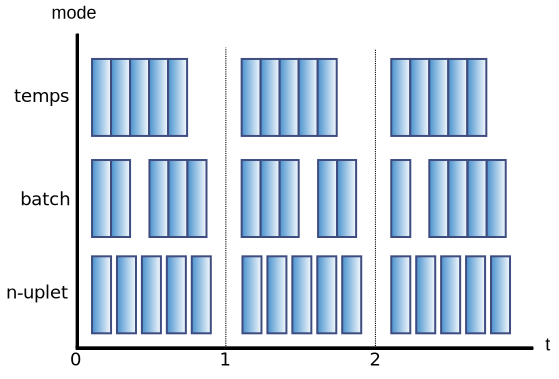
\includegraphics[width=0.75\textwidth]{rw-sgfd-modes}
    \caption{Représentation des différents modes d'exécution des SGFD}\label{fig:rw:sgfd:modes}
\end{figure}
L'unité de temps n'est donc pas le \textit{timestamp} ou l'n-uplet, ce sont les batchs. D'un point de vue physique, cela correspond à un \textit{envoi groupé} de la part de la source.
\begin{example}
 Une source d'événement produit un flux d'information. Si deux événements se produisent au même \textit{instant} (à l'unité de temps près)\footnote{Ces cas apparaissent facilement dans les cadres de grande échelle ou lorsqu'un événement est cause d'un autre}, la source effectuera quand même deux actions de production de la source, ces productions correspondent aux batchs.
\end{example}

Par la suite, des opérateurs sont développés pour manipuler les batchs pour passer d'un mode d'exécution à l'autre. Par exemple, il est possible de structurer les batchs d'un \textit{timestamp} donné à partir d'un autre attribut (identifiant par exemple).

De façon similaire, nous pouvons effectivement remarquer que dans l'algèbre \textit{ACO} la gestion de l'ordre positionnel est flou Le flux est ordonné par \textit{timestamp}, mais en cas de n-uplets dits \textit{simultanés}, aucun ordre strict n'est définit. Dans la définition de la fenêtre positionnelle, \textit{ACO} introduit la définition d'une suite $(s_n)$ strictement ordonnée. A. Arasu a dit sur ce point dans son manuscrit de thèse : \enquote{\it Comme nous ordonnons arbitrairement la séquence $s_1$, $s_2$,..., les fenêtres positionnelles sont non-déterministes lorsque les \textit{timestamps} ne sont pas uniques, ce qui peut ne pas être approprié}. L'introduction apporte donc une généralisation de l'ordre temporel, ce qui peut permettre d'empêcher certains cas. Toutefois, s'il est nécessaire de sélectionner un nombre limité comme dans l'exemple~\ref{ex:rw:sgfd:batches}, le choix reste non-déterministe.

Suite à l'identification des problèmes de modes d'exécution, le modèle \textit{SECRET} a été développé. Le principe étant de décomposer l'opérateur de fenêtre en trois parties. Tout d'abord, le modèle décrit sa portée et son contenu (\textit{scope \& content}) pour savoir quels n-uplets seront inclus dans les fenêtres. Ensuite, les auteurs détaillent son mode de consommation d'n-uplet (\textit{tick}), et enfin son mode de notification à l'utilisateur. Cette séparation claire des concepts permet d'avoir une meilleur compréhension des sémantiques possibles sur les fenêtres. Ainsi, ce modèle permet de décrire les modes de fonctionnement de systèmes existants pour mieux permettre leur intégration par la suite.

Enfin, les travaux de Krämer~\cite{Kramer:semantics} détaillent une algèbre de manipulation des flux, le point novateur étant le fait de séparer l'aspect brut, logique et physique. Les flux tels que nous les avons décrit dans cette section sont des flux bruts composés de couples $(\textrm{n-uplet},\textit{timestamp})$. Les flux logiques sont quant à eux un ensemble de triplets $(\textrm{n-uplet}, \textit{timestamp}, n)$. La multiplicité $n$ permet de compter le nombre d'occurrences du n-uplet a été observée dans le flux originel. Les flux physiques utilisent eux une définition très similaire à ce qui peut se trouver dans les bases de données temporelle avec un intervalle de validité. Ses élements sont donc des couples $(\textrm{n-uplet},[t_s, t_e[)$. Deux algèbres sont ainsi décrites, l'une pour les flux logiques (manipulés pour la sémantique) et l'autre pour les flux physiques (manipulés par l'implémentation). Des équivalences d'expressions sont ensuite définies pour manipuler ces notions.

\subsection{Synthèse}
Beaucoup de modèles théoriques ont été spécifiés lors de ces 15 dernières années pour gérer les flux de données. La sémantique est de plus en plus claire pour la plupart des opérateurs même complexes. Les premiers résultats d'équivalences de requêtes ont pu voir le jour. Toutefois, certains points sont encore manquants :
\begin{itemize}
 \item[\textbf{Le fenêtrage}] : malgré les efforts récurrents de formalisation de cet opérateur, la sémantique reste souvent restreinte à la fenêtre glissante. Qu'en est-il des fenêtres moins conventionnelles mélangeant à la fois les positions et le temps ? Ce type de fenêtre apparait pourtant dans des systèmes d'observations \textit{fenêtre sur 5 données, toutes les 3 minutes}.
 \item[\textbf{L'ordre}] : comme nous l'avons présenté, certains traitement considèrent que des résultats peuvent être non-déterministe. Cet aspect montre un caractère aléatoire qui peut ne pas être de rigueur. Quels sont les conséquences si des ordres plus stricts sont imposés ?
 \item[\textbf{La synchronisation}] : les algèbres manipulent une requête avec un \textit{timestamp} de départ $t_0$. Si ce \textit{timestamp} est altéré la sémantique finale ne sera pas la même, rendant ainsi le partage des résultats plus délicat.
 \item[\textbf{Les équivalences}] : plusieurs équivalences de requêtes simple existent déjà. Toutefois, elles sont souvent remises en question avec des modèles plus expressifs. Comme les équivalences de requêtes sont la pierre angulaire pour permettre une optimisation logique, il est nécessaire d'investiguer sur ce point.
 \item[\textbf{Le couplage relationnel}] : il a toujours été supposé possible de faire des jointures avec des \textit{relations statiques} dans les algèbres. Toutefois, les relations issues d'SGBD ne sont pas statiques dans le temps. La prise en compte des mises à jours dans le modèle est crucial pour permettre d'effectuer le couplage SGBD-SGFD que nous avons mentionné en conclusion du chapitre~\ref{chap:rw:supervision}.
\end{itemize}


\section{Infrastructure de traitement}\label{sec:rw:sgfd:infra}
La structure interne des systèmes de gestions de flux de données diffère entre les implémentations. Toutefois, plusieurs concepts fondateurs sont couramment utilisés pour permettre l'exécution correcte des requêtes. Tout d'abord, nous présentons les principes des infrastructures des SGFD. Ceux-ci sont fondamentaux pour permettre l'intégration de systèmes hétérogènes. Ensuite, nous détaillons les principes architecturaux développés particulièrement pour permettre aux infrastructures de supporter les grandes quantités de données.

\subsection{Du modèle vers l'implémentation}
Le modèle théorique permet de formaliser la sémantique exacte des expressions de requêtes. La mise en œuvre de ces expressions est plus délicate. La connaissance de cette structure est nécessaire non seulement pour comprendre le fonctionnement des SGFD. Mais de plus, cela permet la mise en œuvre de solutions de médiations de systèmes~\cite{Tatbul:integration}.

\subsubsection{Les résultats intermédiaires}
Comme présenté précédemment en section~\ref{sec:rw:supervision:datastream}, la gestion de flux de données se décompose en trois composants principaux : les sources, les opérateurs et les puits. Les opérateurs consomment une ou plusieurs entités (un flux par exemple) et produisent une nouvelle entité. Ces entités sont matérialisés par des résultats intermédiaires comme présenté dans la figure~\ref{fig:rw:sgfd:modeleimplem}.
\begin{figure}[ht]
    \centering
    \includegraphics[width=0.8\textwidth]{rw-sgfd-modeleimplem}
    \caption{Implémentation d'un opérateur avec les résultats intermédiaires}\label{fig:rw:sgfd:modeleimplem}
\end{figure}

Ces résultats intermédiaires utilisent des mémoires tampons (et occasionnellement des supports persistants~\cite{Abadi:aurora}). Ces résultats sont manipulé par une interface d'appel très simple en général basé sur les primitives \textit{push} et \textit{pop} telle une pile. Leur fonctionnement peut toutefois être plus compliqué en introduisant des primitives d'ordres ou de sélection comme dans les \textit{SweepArea} de \textit{PIPES}~\cite{Kramer:semantics}. Le point crucial de la gestion de flux de données est de maîtriser ces canaux.

\subsubsection{L'exécution}
Deux types d'exécutions sont référencés : les non-bloquantes et les  bloquantes~\cite{Babcock:issues}. Originellement, un opérateur \textit{bloquant} est \enquote{\it un opérateur qui n'est pas capable de produire son premier n-uplet tant que l'ensemble de son entrée n'a pas été consommé}. Les opérateurs souvent cités sont les agrégats. Par la suite, grâce aux recherches sur les fenêtres~\cite{Maier:semantics}, le terme est généralisé aux opérations de fenêtrages dont le décalage est différent de \textit{1 n-uplet}.

Ainsi, les opérateurs blocants ne sont pas seulement cadencés par le donnée de son entrée. Ils ont leur propre cycle de vie, ce qui les rend plus compliqués à exécuter. Le module d'ordonnancement (\textit{scheduler})~\cite{Carney:scheduling} est donc présent dans la plupart des implémentations supportant ce type d'opérateur. Ce composant a pour tâche de décider quel opérateur exécuter et quand.

Quant à la communication entre les canaux et autres modules, les mécanismes de souscriptions (\textit{publish/subscribe} ou \textit{push})~\cite{Eugster:publishsubscribe} ne sont pas toujours adoptés. En effet, au lieu d'appliquer strictement l'approche événementielle, l'infrastructure peut nécessiter de privilégier une approche par appel (\textit{pull}). 

Par exemple, le moteur MXQuery~\cite{Botan:MXQuery} est un SGFD dont la particularité est de traiter des documents \textit{XML} tels que \textit{RSS} (flux d'actualités). Ce moteur ne supporte que l'approche \textit{pull} en entrée. A la différence, un SGFD plus généraliste tel que STREAM supportera un mécanisme événementiel. La gestion de l'hétérogénéité de la dynamique des données s'applique donc aussi au niveau de l'infrastructure d'exécution des requêtes.

\subsubsection{Intégration de systèmes}
Comme nous l'avons présenté, les implémentations de SGFD diffèrent en terme d'architecture, de modèle de données, de langage de requête et même de paradigme d'exécution. En ce sens, le système Exoengine~\cite{Duller:virtualdsms} virtualise les éléments qui composent un SGFD quelconque. L'implémentation de celui-ci se fait dans l'architecture à service. Ainsi, les divers canaux exposent deux interfaces de services, l'entrée et la sortie. Il devient désormais possible de relier naturellement des canaux entre eux afin de gérer le flot des données pour les unir ou les disperser vers plusieurs unités de traitement.

\begin{figure}[ht]
    \centering
    \includegraphics[width=0.8\textwidth]{rw-sgfd-virtualslet}
    \caption{Un \textit{slet} virtuel permettant d'abstraire le fonctionnement d'un SGFD}\label{fig:rw:sgfd:virtualslet}
\end{figure}
Par la suite, il est nécessaire de créer des encapsulations du système originel pour s'adapter à ces interfaces de services. La figure~\ref{fig:rw:sgfd:virtualslet} montre une telle manipulation. La puissance d'une telle approche est non seulement de pouvoir gérer l'hétérogénéité des systèmes, mais aussi de pouvoir :
\begin{itemize}
	\item Rendre un système distribuable. En implémentant des canaux réseaux dont l'entrée est sur une machine et la sortie sur une autre, il devient possible d'avoir une communication entre deux systèmes distribués. L'utilisation du même système sur plusieurs nœuds réseaux permet la distribution du calcul bien que le moteur originel ne le supporte pas.
	\item Convertir un système \textit{pull} en système \textit{push} et inversement. L'hétérogénéité des mécanismes est donc gérée grâce à l'abstraction de service car les canaux supportent les deux modes de fonctionnements.
	\item Utilisation de plusieurs modèles de données. Les canaux transmettent des objets avant tout, celui-ci peut être la représentation d'un \textit{XML} ou d'un n-uplet relationnel. En ajoutant des \textit{slets} de conversions, il est possible de faire fonctionner deux moteurs différents ensemble.
	\item Remplacement d'un composant à chaud. L'utilisation de l'approche à service permet aussi une bonne gestion du cycle de vie des composants. Ainsi, l'administration des requêtes et des composants (\textit{slets} ou canaux) peut se faire pendant que le système est en fonctionnement.
\end{itemize}

Toutefois, la médiation de système n'est valable que d'un point de vue infrastructure. En effet, la mise en œuvre entre les différents systèmes suppose que l'utilisateur est capable de traduire la sémantique de sa requête sur chaque système. Or, nous avons vu qu'il n'existe pas de langage universel permettant de traduire la sémantique de chacun des systèmes pour tous ses aspects.

\subsection{Passage à l'échelle}
L'architecture des SGFD s'est beaucoup concentré sur son passage à l'échelle notamment en terme de volume. En effet, l'intégration des SGFD et des réseaux de capteurs notamment a permit le développement de nouvelles architectures. En effet, les réseaux de capteurs sont capables de se gérer à une portée limité du fait de leur contrainte de puissance et d'énergie. A contrario, les SGFD sont capables de traiter les données sur tout type de plateforme. C'est ainsi que lorsque le nombre de sources s'intensifie des goulots d'étranglements peuvent se créer.

\subsubsection{Architecture distribué}
La distribution de l'architecture pour passer à l'échelle fait parti des techniques classiques. La structure même des requêtes en forme d'arbre d'opérateur permet la mise en œuvre naturelle de structures hiérarchiques. En effet, des systèmes tels que \textit{Borealis}~\cite{Abadi:borealis} (historiquement, l'évolution d'\textit{Aurora}) permettent de distribuer le calcul d'une requête sur plusieurs nœuds avec toutes les complications que cela implique.

La distribution d'un calcul emmene les problématiques de synchronisation, de répartition de charge, des tolérances aux fautes et de latence de traitement. Des recherches~\cite{Hwang:distributed, Tucker:heartbeat} ont donc été faites sur ce point pour permettre une évaluation exacte avec une latence faible pour garantir un traitement rapide.

L'approche hiérarchique permet de faire du traitement à plusieurs niveaux. Ces niveaux peuvent avoir un rôle bien défini dans le traitement des données. C'est le cas pour \textit{HiFi}~\cite{Franklin:hifi} présentant cinq niveaux de traitement des données. À chaque niveau correspond un type d'opération et à une localisation bien défini :
\begin{itemize}
	\item[\textbf{Nettoyage} :] Application de filtres sur les données pour enlever les anomalies. Traitement situé sur le capteur.
	\item[\textbf{Lissage} :] Interpolation des mesures perdues. Utilisation d'agrégats sur les fenêtres. Traitement situé sur la station d'accueil des capteurs.
	\item[\textbf{Arbitrage} :] Consolidation des données. Suppression de données dupliquées, agrégations des données nécessaires au niveau suivant. Traitement situé au niveau d'un batiment.
	\item[\textbf{Validation} :] Applications de règles métiers pour valider les données. Utilisation principale de jointures. Traitement situé à un niveau régional.
	\item[\textbf{Analyse} :] Support de décisions tels que vu dans la section~\ref{sec:rw:supervision:warehouse}. Traitement situé au centre de commandement.
\end{itemize}

Cette approche a été généralisé dans \textit{SStreamWare}~\cite{Gurgen:sstreamware} avec les \textit{sites de contrôles} (plus haut niveau hiérarchique) et les \textit{passerelles}. Ces dernières sont capables d'accueillir des capteurs (virtuels ou non), ainsi que d'exécuter une requête de flux sur les capteurs accueillis ou sur des flux externes venant d'une autre passerelle. Le site de contrôle est celui qui distribuera la requête sur les différentes passerelles.

\subsubsection{Désignation}\label{sec:rw:sgfd:infra:designation}
Plus le nombre de sources augmente, plus il devient difficile de maîtriser lesquelles sont concernées par la requête que l'utilisateur souhaite déployer. Une requête par désignation est une requête utilisant une autre requête pour désigner les sources de données à lire. Par exemple : \enquote{\it Le flux des mesures des capteurs de température du batiment A}. Dans cette requête, il est nécessaire de d'abord faire une interrogation sur l'expression \enquote{\it Quels sont les capteurs situés dans le batiment \textit{A} et de type \textit{température}} avant de déployer la requête.

Ce procédé est naturellement implanté dans notamment SStreamWare, HiFi et GSN~\cite{Aberer:gsn}. L’objectif à long terme de ce dernier est de former un internet de capteur. Son architecture est donc naturellement pair-à-pair. L’interrogation continue sur ce système peut se faire par le déploiement d’un nouveau capteur virtuel. La désignation est donc centrale, car la formation d’un capteur virtuel à partir d’autres sources est possible. Toutefois, du fait de l’absence de méta-données la puissance d'expression de cette requête de désignation est limité. Dans SStreamWare et HiFi, au contraire, le support des méta-données telles que son lieu, son type ou sa fréquence d'émission permet de correctement sélectionner les sources concernés.

\subsection{Synthèse}
L'infrastructure des SGFD a reçu beaucoup d'attention en terme d'architecture, de tolérance aux fautes, d'intégration et de support des multi-échelles. Le point crucial manquant reste encore la compréhension de la sémantique des requêtes. En effet, lors de l'intégration des systèmes, qui est la pierre angulaire de la compréhension des infrastructures, nous avons vu qu'il était nécessaire que l'utilisateur sache traduire l'expression de ses sous-requêtes dans les différents langages. De plus, du fait de l'ambiguïté sémantique de l'exécution des différents opérateurs tels que nous l'avons décrite dans la section~\ref{sec:rw:sgfd:modeles}, l'expression de ces requêtes peut porter à confusion. De façon similaire, le procédé de désignation semble limité en pouvoir d'expression. Son exécution, en terme d'infrastructure, est limité car, par définition, l'exécution d'une requête en implique une autre avant son déploiement. Une généralisation de cette approche est donc nécessaire.
\section{Intégration de supports persistants}
Les supports persistants sont dirigés par le paradigme de l'interrogation instantanné. Bien que les gestionnaires de bases de données et de flux de données partagent les mêmes fondations théoriques. Le problème réside dans la difficulté à combiner les deux paradigmes : requêtes continues sur des flux continus et requêtes instantannées sur une base de donnée.

\subsection{Requêtes dépendantes à un contexte}
Nous avons déjà vu les requêtes par désignation dans la section~\ref{sec:rw:sgfd:infra:designation}. La requête sous-jacente utilisée pour désigner les sources d'informations est posée sur un ensemble de donnée de manière instantanné. Nous retrouvons donc un cadre similaire. L'ensemble des données pouvant être interrogé par cette requête est assimilable à un contexte tel que présenté en section~\ref{sec:rw:supervision:context}.

L'utilisation d'un catalogue de meta-données en tant que contexte est souvent utilisé dans les applications de supervisions à base de flux. Cette utilisation a été pratiqué dans les projets SStreamWare et plus récemment sur SmartCIS~\cite{Liu:smartcis}. Dans ce dernier, un SGBD relationnel est utilisé pour recenser les différents dispositifs logiques et physiques. Au moment du déploiement de la requête, l'optimiseur interroge cette base de donnée pour sélectionner les sources. D'un point de vue modélisation, les méta-données sont considérés comme des attributs spéciaux des flux. Lors de la réécriture de la requête, les attributs de méta-données sont écartés pour effectuer l'interrogation sur le catalogue. Il est intéressant de noter que la dynamique des meta-données est typiquement \textit{stable} ou \textit{statique}.

Toutefois, le contexte peut être mis à jour. L'impact d'une telle mise à jour influera sur l'évaluation de la requête. Par exemple, si l'utilisateur déploie la requête précédemment citée : \enquote{Flux des températures du batiment A} et qu'un nouveau capteur arrive dans le batiment. Doit-il être pris en considération ? Cette idée ouvre la voie au concept de transaction dans le cadre des requêtes continues. Le phénomène a d'abord été cerné et répondu par le protocole de mise à jour de SStreamWare~\cite{Gurgen:transaction}. Si une mise à jour est effectuée, le protocole ira modifier les nœuds et les requêtes concernés pour changer le déploiement si nécessaire.

De façon proche, l'idée de transaction pour les requêtes continues a ensuite été présenté dans~\cite{Botan:transaction}. Les transactions sont définies comme un ensemble restreints d'opérations de lectures ou d'écritures appliquées sur les flux ou relations avec un ordre d'exécution défini. De cette façon, l'exécution de requête continues est un ensemble de micro-transactions, garantissant une exécution sans conflit. Il est notable que cette conception permet de réutiliser les transactions des gestions bases de données.

D'un point de vue opérationnel, la sélection sur méta-données consiste en une semi-jointure (sur les identifiants typiquement) avec le résultats d'une jointure sur un support persistant. Ainsi, soit le système applique une désignation comme vu précédemment, et ouvre la possibilité à des problèmes de sémantiques devant être gérés par des protocoles de mises à jours. Soit, le système applique l'opération de semi-jointure avec le support persistant qui a une vue à jour des données.

\subsection{Analyses sur historique}
%La deuxième utilisation majeure des supports persistants est le fait de 

%The second main usage is gathering logged data from the past of a stream as seen in query Q\ref{query:historicsensor}. The implementation must consider the fact that logged data are constantly augmented and that the aggregate operation may be costly. The first proposal tackles such query is the joint work between FastBit and TelegraphCQ~\cite{Reiss:fastbit}. Two queries were specified from the data stream point of view, and from the log storage point of view. Then, a controller would execute the two queries in order to add data from the logged query for each tuples on the stream.
%
%Later on, a more explicit operator has been defined in Moirae~\cite{Balazinska:moirae}: the operator \textit{Recall}. For a specific identifier, \textit{Recall} gathers aggregates from the history $H$. To absorb the charge, the management of \textit{recall operations} can be distributed. \textit{Materialized contexts} are used to perform semi-joins as seen previously. This allows past data of a stream to be used as meta-data describing this stream.
\subsection{Une première approche intégrée}

%In this section we will see how related works used persistent data along with a data stream management system in order to enhance their monitoring capabilities. 
%Three main ways to deal with queries like Q\ref{query:designation} Q\ref{query:historicsensor} can be identified: the use of catalogs, the use of stream dump and the use of streams inside a DBMS.
%
%\textbf{Using a catalog}: 
%The first main usage consist in appending meta-data from a catalog to the stream e.g. to evaluate Q\ref{query:designation}. A straight-forward solution would be to make the stream source (i.e. sensors in Q\ref{query:designation}) generate all associated meta-data. A more efficient way is to have a \textit{persistent} catalog in order to know if a specific source matches meta-data (e.g. type temperature and inside building \textbf{A}). This usage has been chosen on (X)SStreamWare~\cite{Gurgen:sstreamwarepaper} and more recently on SmartCIS~\cite{Liu:smartcis}. In those projects, the main stream contains specific attributes (called \textit{properties}). If one of them is used in a selection of projection, it is specifically queried from a device catalog potentially spread around the distributed architecture.
%
%However, as shown in~\cite{Gurgen:update}, the impact of changes in the meta-data may affect the query evaluation and semantic. For instance, if a new sensor enters into the building, must its stream be included in the query or not? Such choices are currently mainly dependent on the implementation and are not specified  at the query language level.
%
%From an operational point of view, selecting on meta-data consists of a semi-join (on the identifiers typically) with the result of a query on a persistent support. This allows to select the right sources of data early on (temperature sensors, \textit{and} inside the building A). Two types of implementation have been made for two kinds of architectures. Distributed architectures and sources on different nodes, this selection on meta-data is made during the deployment of the query plan as in GSN~\cite{Aberer:gsn} and HiFi~\cite{Franklin:hifi}. This execution is optimal as it does not call the ignored sources, but if there is any changes on the catalog, the query results will not be updated unless the plan is reconstructed explicitly. The second implementation gathers the data until an operator which will perform the semi-join on an up-to-date view of the persistent data. This approach can be used on centralized DSMS or with shared queries. This is not optimal from a communication point of view but a fresh and consistent view of the meta-data is provided at any time.
%
%\textbf{Performing aggregate of stream dump}: 
%The second main usage is gathering logged data from the past of a stream as seen in query Q\ref{query:historicsensor}. The implementation must consider the fact that logged data are constantly augmented and that the aggregate operation may be costly. The first proposal tackles such query is the joint work between FastBit and TelegraphCQ~\cite{Reiss:fastbit}. Two queries were specified from the data stream point of view, and from the log storage point of view. Then, a controller would execute the two queries in order to add data from the logged query for each tuples on the stream.
%
%Later on, a more explicit operator has been defined in Moirae~\cite{Balazinska:moirae}: the operator \textit{Recall}. For a specific identifier, \textit{Recall} gathers aggregates from the history $H$. To absorb the charge, the management of \textit{recall operations} can be distributed. \textit{Materialized contexts} are used to perform semi-joins as seen previously. This allows past data of a stream to be used as meta-data describing this stream.
%
%\textbf{An integrated alternative}: 
%Finally, Oracle has presented in~\cite{Witkowski:oraclecq} a framework to manipulate continuous queries in the Oracle DBMS. Therefore, stream, relations and logs are in the same system and can be manipulated together. However, the system lacks of a common algebra to formalize the integration of the two worlds. The user has to describe how materialized views must be created and updated. To our knowledge~\cite{Witkowski:oraclecq} is the only work that explicitly presents different semantics for updates of data used by continuous queries. The approach is mainly driven by an implementation point of view. The infrastructure is able to execute queries such as Q\ref{query:designation} and Q\ref{query:historicsensor}. On the theoretical side, some proposals~\cite{Patroumpas:window,Jain:spread} have been made to formalize data stream management. But to our knowledge, no project has yet tackled the issues of handling the instantaneous query paradigm inside a continuous query processing system.
%
%Yet, adopted approaches are mainly driven by implementation of ad-hoc solution driven by specific application needs. 
%But integration, in a non specific way, of both streaming and relational world is an important step for many applications such as the one presented in the next section.

\section{Optimisations}\label{sec:rw:sgfd:optim}
L'héritage des connaissances du domaine des systèmes relationnels a été central sur la conception des systèmes de gestion de flux de données. Concernant l'optimisation du traitement des requêtes, il existe plusieurs techniques concernant les SGBD. Dans cette section, nous présenterons les stratégies d'optimisations appliqués aux SGFD. Tout d'abord, nous rappellerons les grands principes du traitement des requêtes des bases de données. Par la suite, nous nous concentrerons sur les points spécifiques à la nature des requêtes continues. Enfin, nous présenterons des principes d'implémentation des algorithmes spécifiques aux opérateurs.

\subsection{Optimisation dans les SGFD-R}
Ainsi, afin de mieux analyser les optimisations de la gestion de flux, il devient important d'investiguer plus en détail le fonctionnement de la gestion de base de données.

\subsubsection{Le problème dans sa globalité}
Le processus d'optimisation usuel en gestion de base de données est maintenant établie et répendue~\cite{Ioannidis:optimization}. Une requête en gestion de base de donnée est soumise par un langage déclaratif tel que \textit{SQL}. A partir de cette expression, s'enchaine une série d'opération qui permettra l'exécution de celle-ci. La figure \ref{fig:rw:sgfd:optim:processus} décrit le processus complet nécessaire à l'aboutissement de ce traîtement. 
\begin{figure}[h]
\centering
\includegraphics[width=0.9\textwidth]{rw-sgfd-optimsgbd}
\caption{Processus de traitement de requête dans un SGBD-R}\label{fig:rw:sgfd:optim:processus}
\end{figure}

Plusieurs modules permettent d'exécuter cette série d'opérations :
\begin{itemize}
    \item \textbf{Analyseur} : Prend en entrée une requête textuelle et fournit en sortie un arbre de requête écrit dans un format interne équivalent à de l'algèbre relationnelle. Ce module ne fait que traduire la grammaire du SQL par des règles prédéfinies.
    \item \textbf{Optimiseur} : Prend cet arbre de requête et fournit un autre arbre de requête, agrémenté d'indication de méthodes physique à utiliser. Le tout forme une stratégie d'exécution qui ne sera pas modifiée par la suite. Le but de cette étape est de fournir la stratégie qui fournit un résultat identique à ce que l'arbre initial était avec un coût moindre.
    \item \textbf{Interpréteur} : Récupère la stratégie d'exécution et instancie les procédures d'exécution. Le tout sera envoyé à l'\textbf{exécuteur} qui manipulera ces procédures afin de produire le résultat final.
\end{itemize}
L'optimiseur étant bien entendu le module le plus complexe car il possède et utilise beaucoup de connaissance et de résultats sur la gestion de données. Ce composant s'est prouvé indispensable dans la pratique car une bonne stratégie de traitement changera la plupart du temps de complexité ce qui transformera une requête pouvant être exécutée en plusieurs heures en moins d'une seconde.

Le problème est que l'espace des stratégies possibles pour exécuter une requête classique est potentiellement de cardinalité factorielle en fonction du nombre d'opérateurs et de méthodes d'exécutions disponibles (surtout s'il y a des jointures). Ainsi, il faut guider l'exploration et utiliser des techniques de programmation dynamique pour éliminer rapidement les branches trop coûteuses.

L'optimisation de requête se découpe en deux sections : l'optimisation logique (i.e. sélection du meilleur arbre d'opérateur théorique) et l'optimisation physique (choix des meilleurs algorithmes).

\subsubsection{Optimisation Logique}
L'espace algébrique est très large car les équivalences sur l'algèbre relationnelle sont très larges et permissives. Par exemple, une sélection sur une jointure $\sigma (R_1 \Join R_2)$ peut traverser l'opérateur binaire si sa condition ne concerne qu'une branche : $R_1 \Join \sigma R_2$. Ainsi, pour un arbre de requête, il peut y avoir des millions de requêtes équivalentes avec des permutations ou des ajouts d'opérateurs. Des heuristiques sont ainsi sélectionnées pour réduire cet espace tout en restant efficace~\cite{Ioannidis:optimization}. Le critère principal d'optimisation étant minimiser la taille des résultats intermédiaires. Voici les règles classiques :
\begin{itemize}
    \item[\textbf{R1}~:] \textit{La sélection et la projection n'introduisent pas de coût supplémentaires et sont traités à la volée}. Les sélections doivent être exécutés au moment de la première lecture sur la relation. Les projections doivent se faire en même temps que le résultat d'un autre opérateur.
    \item[\textbf{R2}~:] \textit{Les produits cartésiens ne doivent jamais être formés sauf si la requête elle-même en demande}. Seules les jointures peuvent combiner des relations.
    \item[\textbf{R3}~:] \textit{L'opérande interne (partie droite) de chaque jointure est une relation originelle, et non un résultat intermédiaire}.
\end{itemize}

La règle R1 est utilisée pour minimiser la taille des résultats intermédiaires. La règle R2 supprime toute possibilité de recours fatal aux algorithmes de boucles imbriquées sachant qu'un autre plan pouvait utiliser à chaque fois des jointures plus efficaces.

La règle R3 n'est pas toujours choisie car même si elle réduit beaucoup les possibilités car elle restreint les ordres de jointures, elle risque de supprimer l'arbre optimal dans plusieurs cas. En effet, les arbres de requêtes ne pourront pas être des arbres équilibrés car l'opérande droite doit être une relation native, or un arbre déséquilibré peut introduire des surcoûts du fait que les jointures supérieur doivent joindre une grande relation avec un résultat intermédiaire. Toutefois, il existe des raisons à cette règle. Tout d'abord, le fait d'avoir des relations natives permet l'utilisation d'index. De plus elle permet de faire un traitement total des requêtes en mode \textit{pipeline}\footnote{L'exécution en \textit{pipeline} permet de traiter un n-uplet dès sa lecture, notons que cela s'apparente à du traitement de flux. L'avantage étant que le processeur étant moins coûteux que les entrées-sorties, on peut rentabiliser l'attente de lecture en traitement de requête.}.

En parcourant l'espace algébrique des requêtes équivalentes vérifiant R1-3, le nombre de plans devient raisonnablement faible. Pour le reste des recherches, il sagit principalement de choisir l'ordre des jointures. Comme la jointure est symétrique $R_1 \Join R_2 = R_2 \Join R_1$ alors dans le cas de multiples jointures (courant en gestion de base de données), il faut choisir l'ordre le plus pertinent qui minimisera la taille des résultats intermédiaires. Cette recherche se fera conjointement avec l'optimisation physique du fait de son impact sur les algorithmes.

\subsubsection{Optimisation Physique}
L'optimisation physique correspond au parcours de l'espace des méthodes disponibles pour chaque plan de requête et à l'évaluation quantitative de chacune de celles-ci. L'espace des méthodes fournit plusieurs implémentation pour un opérateur. Par exemple pour la jointure :
\begin{itemize}
    \item \textbf{Boucles imbriqués} : Implémentation la plus directe de la jointure. Cet algorithme ne requiert aucune condition sur les relations d'entrées.
    \item \textbf{Jointure fusion} : Se base sur le fait que les deux relations sont triés sur l'attribut de jointure à l'avance. Ainsi la jointure est plus facile à effectuer. Elle est régulièrement utilisée avec des index triés comme les arbres B+~\cite{Comer:btree}. Des opérateurs de tri pourront être déployés si ces index sont absent.
    \item \textbf{Jointure hachée} : Se base sur le fait que les deux relations sont hachées sur l'attribut de jointure. Ainsi la jointure se fait sur les index de hachages de cardinalité réduite et d'accès rapide.
\end{itemize}

Pour chaque relation, il existe deux moyens principaux d'accéder à un n-uplet :
\begin{itemize}
 \item \textbf{Scan} : Parcours strict de la relation ou d'un l'index pour trouver les n-uplets vérifiant une condition de sélection.
 \item \textbf{Probe} : Demande directement aux procédures d'index de renvoyer les tuples vérifiant une condition de sélection.
\end{itemize}

Ainsi, il est possible de faire des boucles imbriqués suffisamment performantes en utilisant des accès optimisés aux relations. Bien évidemment certaines sélections sont impossibles via les procédures d'index. Par exemple, il est impossible de demander à un index haché de faire une sélection avec un opérateur de comparaison tel que \enquote{$\leq$}.

L'évaluation de chacune de ces méthodes passe par un coût global de l'exécution basé sur des statistiques. Ces statistiques aideront à quantifier la taille des résultats intermédiaires. Pour cela, il est nécessaire de faire des calculs de sélectivité~\cite{Selinger:selectivity}. Ces calculs permettent d'évaluer le ratio d'n-uplet qui valident une sélection. Par exemple, en l'absence d'information complémentaire, une sélectivité de 10\% est appliquée par défaut. Par la suite chaque algorithme est capable de quantifier son coût en fonction de ces sélectivités et des cardinalités des entités manipulées.

Suivant les capacités du système et la taille de la requête, le système pourra réordonner les jointures pour optimiser les algorithmes. La recherche dans cet espace de méthode se base sur la programmation dynamique. Elle permet de faire une recherche exhaustive sans être extrêmement coûteuse (par des procédures de \textit{branch \& bound} usuelles).

\paragraph*{Optimisation de la recherche}
La recherche exhaustive peut être très coûteuse si les jointures sont nombreuses car l'espace des stratégies devient large, ce qui peut être long à calculer. Une approche heuristique est nécessaire pour avoir un temps de calcul qui permette un lancement rapide de la requête. 

Plusieurs approches existent, la plus connue reste basée sur la marche aléatoire sur le graphe des stratégies possibles. Celle-ci parcourt le graphe aléatoirement en reculant si le coût est devenu trop important. Une autre approche intéressante étant l'utilisation d'algorithmes génétiques pour résoudre ce problème. \textit{Postgres} utilise l'optimiseur \textit{Genetic Query Optimizer (GEQO)}~\cite{Postgres:geqo} si le nombre de jointure dépasse une certaine limite.

L'optimisation a été prouvée comme un problème NP-complet~\cite{Ibaraki:join} (même avec seulement les boucles imbriqués) ainsi certains efforts se sont concentré sur la résolution de sous cas importants, notamment boucles imbriqués et jointure hachée seulement.

\paragraph*{Base de données parallèles}
L'optimisation en prenant en compte des modèles de calculs parallèles est un problème encore ouvert. Toutefois, des approximations efficaces se basent sur les optimisations à deux phases. Tout d'abord, le système recherche la solution optimale comme vu précédemment. Par la suite, il cherche le meilleur ordonnancement. Les deux domaines ont été suffisamment couverts pour obtenir des résultats satisfaisants.

\paragraph*{Distribution du calcul}
La distribution du calcul est un problème différent des bases parallèles dans le sens où il existe plusieurs unités d'évaluation complètement indépendantes. Le problème toutefois se résout principalement en quantifiant la distribution du calcul à l'intérieur de l'espace des méthodes. L'espace de recherche sera toutefois plus grand et il faudra faire attention à avoir un optimiseur performant pour ne pas avoir de surcoût avant l'exécution.

\paragraph*{L'optimisation sémantique}
Supposons la présence d'une base de connaissance en parallèle de la base de donnée. Il est alors possible de raisonner sur les conditions de sélections notamment, afin d'amener plus ou moins de restriction à la requête. Les calculs d'inférence de concepts, comme vus en section~\ref{sec:rw:supervision:contexte}, permettent d'extraire des conditions plus restrictives mais équivalentes. Le problème étant d'avoir une base de connaissance suffisamment exploitable car une erreur de raisonnement pourrait supprimer potentiellement des résultats. De plus, les calculs d'inférences peuvent être lourds et ne doivent pas rendre le traitement de requête trop lourd. Cette approche commence a être exploitée en gestion de flux de données aussi grâce à des méta-données~\cite{Ding:semantic}.

\subsection{Optimisation spécifique de la gestion de flux}
L'infrastructure de traitement des flux est sensiblement différente à la gestion des bases de données. Ainsi, des optimisations plus spécifiques sont applicables dans ce contexte concernant : le mode de traitement des requêtes, la gestion de la charge sur le long terme, le partage des requêtes, l'ordonnancement et enfin le routage pour les infrastructures distribués. Nous pouvons remarquer que toutes ces optimisations ont été explorées premièrement dans le domaine des systèmes de base de données. Toutefois, ils prennent plus d'ampleur dans ce contexte.

\subsubsection{Calcul incrémental}
Le principe fondateur de la gestion de flux étant que les données arrivent de manière continue. Comme présenté dans la section~\ref{sec:rw:sgfd:modeles}, les premiers traitement de flux~\cite{Terry:tapestry} étaient considérés comme des traitements particuliers sur des relations sans suppression ou mise à jour.

De façon plus générale, en se plaçant dans l'algèbre \textit{ACO} : Soit $R$ une relation, au lieu de calculer une requête sur $R(\tau)$, il est possible de considérer les \textit{delta} de cette relation : $\Delta_R^+(\tau) = R(\tau)-R(\tau-1)$ et $\Delta_R^-(\tau) = R(\tau-1)-R(\tau)$. Comme le traitement des fenêtres, par exemple, peut fournir directement ces différences : il n'y a donc pas de surcoût à l'utilisation d'un tel procédé. Comme la cardinalité des $\Delta$ est souvent minime face à celle de la relation totale. Il devient intéressant de travailler avec ces données.
\subsubsection{Load-shedding}
Contrairement aux approches classiques de gestion de base de données, il est important de voir que l'optimisation n'est pas toujours de pouvoir fournir les résultats exacts aux requêtes. L'objectif étant de fournir les résultats les plus pertinents possibles avec des contraintes d'espace mémoire, de temps de réponse ainsi que de charge réseau. En effet, comme la gestion de flux fonctionne de manière continue, une congestion dans le processus de traitement impliquera des retards et des complications pouvant aller jusqu'à une saturation du moteur.

L'idée du \textit{load-shedding} est de pouvoir abaisser ou limiter le taux de n-uplet au nombre suffisant pour pouvoir traiter sans introduire de retard. Dans les travaux fondateurs~\cite{Tatbul:window,Tatbul:load-shedding}, l'idée est de pouvoir surveiller le traitement des requêtes afin de reconnaitre les points d'engorgements et d'y implanter des opérateurs de shedding. Afin de garantir un certain taux de réussite, la politique qui sera utilisée pour le \textit{load-shedding} sera dirigée par une \textit{QoS}\footnote{QoS : Quality of Service} déterminant quelles données sont utiles. En effet, en prenant en entrée un graphe représentant \textit{valeur} $\mapsto$  \textit{taux de suppression acceptable}. Par exemple, dans le cadre d'une surveillance d'incendie, le taux de \textit{shedding} pour les températures inférieure à 20ºC pourra être très fort de part et d'autre du systèmes pour ce genre de données. Le critère de sélection afin d'autoriser la suppression d'une données peut se faire de façon différentes :
\begin{itemize}
 \item Par un histogramme et un choix sur le nombre de tuple résultant~\cite{Han:join}
 \item Par un calcul probabiliste pour privilégier un flux plutôt qu'un autre pour sa productivité~\cite{Han:join}
 \item Par des raisonnements sur l'age du n-uplet~\cite{Srivastava:join}
\end{itemize}


\subsubsection{Multi-Query Optimization (MQO)}
Aussi connu sous le nom de \textit{Global Query Optimization}. Cette optimisation profite des exécutions parrallèles pour éviter la redondances de traitement et une économie de ressources. Elle est issue du monde des SGBD~\cite{Sellis:mqo} et permet de répondre à plusieurs requêtes en même temps en utilisant des parties communes (classiquement, lorsque seules les clauses de sélection sont différentes). L'idée est toutefois peu exploitée car il faut pouvoir soumettre plusieurs requêtes en même temps et les gestions de caches ont permis de faire de bon résultat pour ce genre de requêtes. 

Dans le monde des flux de données, cette optimisation est largement reconnue comme importante. Les requêtes durant dans le temps, de façon potentiellement infinie, le nombre d'exécution concurrente sera donc très grand. Ainsi, partager les ressources des requêtes devient une façon d'optimiser grandement les requêtes. Plusieurs points interviennent ici.
\begin{itemize}
 \item Tout d'abord l'existence des \textit{m-op} (multi-operators)~\cite{Hong:mqo}. Ces opérateurs permettent de regrouper plusieurs opérateurs en un seul permettant d'éviter des duplicatas de n-uplets. Un exemple classique étant de grouper deux sélections sur un flux commun en une seule. Ainsi, si un n-uplet vérifie les deux sélections, un seul n-uplet sera fournit avec l'indication qu'il appartient aux requêtes 1 et 2. Cette optimisation permet de faire des requêtes en utilisant les définitions de flux fragmentés.
 \item Grande disponibilité des ressources. Chaque opérateur utilise des ressources et peut potentiellement les partager avec d'autres. Cependant, ces ressources ne sont peut-être pas utiles à partager car elles sont trop précises. Dans plusieurs travaux~\cite{Arasu:resource}, le calcul des agrégations sur fenêtres peut être partagé. En découpant la mémoire par bloc de façon intelligente, on peut partager les ressources afin d'économiser de la place mémoire.
\end{itemize}

Un problème ouvert reste de savoir si les optimisations locales (optimisation algébrique) gêneront les optimisations globales. Une requête ne possède pas qu'une seule optimisation au début de son traitement. En effet, si une nouvelle requête arrive et qu'en changeant légèrement la structure de la première, il est possible d'obtenir un partage, alors il est probable que ce nouveau plan soit le bon. L'adaptabilité d'une requête est donc importante.

\subsubsection{Ordonnancement}
Comme les requêtes s'exécutent en parallèle, la notion d'ordonnancement entre en compte. Afin d'éviter les engorgements, ou pour donner plus de priorité à une partie de la requête, l'ordonnanceur doit cadancer les unités de traitement pour fournir des résultats conformes à la qualité attendue. Par exemple, une requête importante (type alerte) peut exprimer des contraintes forte de \textit{latence}. A l'inverse, une requête d'observation passive aura des contraintes plus faible. Plusieurs stratégies ont été proposés~\cite{Babcock:chain, Jiang:scheduling} afin de garantir le meilleur temps de réponse en utilisant le moins de resources possibles.

\subsubsection{Routage}
Le problème du routage est un problème très connu du domaine des réseaux de capteurs où les contraintes de traitement sont si fortes au niveau de la transmission de données que les routages sont importants. Pour le traitement en flux de grandes quantités de données, des optimisations de routages rentrent en compte sur le calcul de jointure par exemple~\cite{Zhou:pmjoin}. En effet, il nous faut savoir s'il vaut mieux effectuer une opération lourde et ayant une sélectivité peut-être grande (>1) de façon distribuée avec transfert réseaux ou groupés mais plus chargés en traitement. 

De façon similaire, le coût (notamment énergétique) est analysé afin de fournir un routage au moment du placement de la requête~\cite{Galpin:snee} ou à l'exécution~\cite{Madden:tinydb}.

\subsection{Optimisation d'algorithmes}

\subsubsection{Jointures}
Comme présenté précédemment, la jointure en flux n'est pas aussi simple qu'une jointure au sens base de données car elle introduit la notion de fenêtre. Beaucoup de travaux~\cite{Han:join, Srivastava:join, Law:join} se sont portés sur les jointures similaires à $I_S (S_1[W_1] \Join ... \Join S_n[W_n])$ et bien souvent avec des fenêtres identiques. Car l'implémentation de ceci requiert a priori une quantité non bornée de mémoire. De plus le traitement d'un n-uplet prendra du temps et il faudra pouvoir fournir le résultat sans retard par rapport aux flux d'entrées. L'utilisation des procédures de \textit{load-shedding} est aussi utile dans ce cas.

L'utilisation d'index, comme couramment appliqué en SGBD, est désormais plus délicat car les données sont constamment actualisées. Le point crucial de l'index étant que le surcoût introduit au moment de l'insertion d'une donnée est amorti par le nombre de fois où la donnée sera interrogée. Il est toutefois important de noter que les optimisations présentes dans le calcul de jointures relationnelles en mode \textit{pipeline}~\cite{Gajski:pipeline} sont ici applicables telles que le \textit{symetric hash join}~\cite{Wilschut:symetricjoin} souvent appliqué.

D'autres optimisations ont été abordés sur la distribution du calcul~\cite{Zhou:pmjoin}. En effet, le coût engendré par les échanges fait que le calcul de la distribution des opérateurs devient importante. Dans cette optimisation, il est important de prendre en compte le partitionnement de la charge du flux par rapport au domaine des attributs de jointures. En effet, un attribut pourra avoir un débit très faible sur une valeur comparé à un autre qui sera bien plus présent.

Enfin, de façon un peu plus particulière, il est intéressant de noter les optimisations dans des contextes particuliers tels que le P2P (avec une DHT)~\cite{Palma:p2p}. Le calcul de la jointure peut se faire sur plusieurs noeuds afin de mieux distribuer le traitement.

\subsubsection{Fenêtrage et agrégations}
Nous nous intéressons maintenant particulièrement aux traitements de requêtes d'agrégations de classe $I_S(G(S[W]))$. Les travaux les plus conséquents se focalisent sur le fait de calculer de façon approximative des opérations de comptage et de quantile en mémoire limité~\cite{Arasu:window}. Ce comptage permet d'effectuer les autres statistiques en quantité restreinte~\cite{Datar:stats}, comme par exemple : 
\begin{itemize}
 \item Min/Max/Sum/Avg 
 \item Moyennes
 \item Tables de hachages
 \item Histogrammes
 \item Nombre de valeurs distinctes
\end{itemize}

L'approche est principalement mathématique et probabiliste. Par exemple, en se fixant une tolérance $\eps$, il est possible d'obtenir un résultat dans une quantité de mémoire prévisible.

L'évaluation exacte efficace de ces opérations reste possible grâce à l'utilisation de \textit{Pane}~\cite{Li:pane}. Le principe étant qu'une fenêtre sur 4 minutes décalée de 1 minute est en fait 4 blocs de 1 minutes. Ces blocs peuvent être agrégés. Ainsi, lors du slide, il sera possible de réutiliser les résultats de chacun de ces blocs pour calculer le résultat de la fenêtre entière. Afin de faire ces opérations, il est nécessaire de catégoriser les fonctions agrégations. 

Les \textit{holistiques} sont définies par deux fonctions $L$ et $S$. Le calcul d'un tel agrégat $F$ sur un ensemble $X$ partitionnés en blocs $(X_n)$ sera fait par : $F(X) = S(\{L(X_i), i\in \N\})$. Dans ce cas, il devient évident que le calcul de l'agrégat sur les fenêtres sera fait par l'application de la fonction $S$ sur les évaluations des blocs par $L$. Par exemple, l'opérateur \textit{max} est \textit{holistique} car $L=S=\max$ est une matérialisation des fonctions. 

Les \textit{différentiables} sont elles définies par trois fonctions $H$, $J$ et $L$ permettant la suppression et l'ajout : $F(X-Y) = H(L(Y), L(X))$ et $F(X\cup Y) = J(L(Y), L(X))$. Par exemple, le comptage et la moyenne sont des opérations \textit{différentiables}. Dans le cadre du comptage $L=$ \textit{count}, $H=-$ et $J=+$ permet de fournir le résultat. Son application dans le cadre de l'évaluation de fenêtre est le fait de reprendre le résultat de la fenêtre précédente, de lui soustraire le bloc qui a été enlevé de la fenêtre, et de lui ajouter le bloc supplémentaire.

\subsection{Synthèse}
Profitant des caractéristiques particulières en terme de contraintes de rapidité d'exécution, il y eu de nombreux développement concernant l'optimisation dans les SGFD. Les plus gros efforts se sont concentrés sur le calcul d'algorithmes incrémentaux, ainsi que sur l'utilisation de réponses approximatives. Seulement quelques approches comme~\cite{Galpin:snee,Kramer:semantics} s'intéressent au fait de faire une optimisation de plan de requête logique puis physique. Toutefois, le manque de connaissance dans le domaine théorique de la gestion de flux de données fait que les équivalences de requêtes sont peu nombreuses en dehors des usuelles~\cite{Slivinskas:temporal,Arasu:stream}.

Ainsi, comparé à l'optimisation des SGBD, seules les règles évidentes telles que l'application de projections au plus près des sources sont faites dans l'optimisation logique. Peu de parcours de plans de requêtes et de stratégies d'exécutions équivalentes n'est appliqué. De même, la prise en considération des autres requêtes pour le partage de résultats intermédiaires est une stratégie efficace. Toutefois, cette opération est principalement faite de façon manuelle à l'installation d'une nouvelle requête. Seuls des travaux comme RUMOR~\cite{Hong:mqo} recherchent à fusionner le nouveau plan de requête avec un autre (sous condition très strictes).

Nous pouvons donc conclure que l'optimisation en gestion de flux de données a été grandement travaillée et a produit de multiples techniques. Toutefois, une utilisation de ces techniques pour faire une \textbf{recherche d'optimisation globale} sans intervention de l'utilisateur est encore limitée notamment du au manque de connaissance théorique.

\section{Conclusion}
Après 20 années de recherche, la gestion de flux de données devient désormais suffisamment mature pour être appliqué massivement. Plusieurs produits commerciaux sont d'ailleurs maintenant utilisés en production. Toutefois, nous pouvons nous rendre compte que la complexité théorique de ces systèmes a été sous-estimé. De nombreux modèles ont été décrit pour représenter les flux de données et leurs traitements. Ces modèles sont encore remis en questions aujourd'hui au fur et à mesure des applications concrètes. 

Nous avons vu que le problème d'avoir une bonne connaissance du modèle et du comportement théorique des SGFD est crucial. En l'état, l'intégration des supports persistants reste ad-hoc et assisté par l'utilisateur. Un fonctionnement intégré avec une modélisation générique capable de gérer les deux modes d'interrogations de façon unifiée est donc indispensable pour manipuler correctement flux et relations persistantes. Similairement, les contributions sur l'optimisation de traitement des requêtes sont encore principalement ponctuelles. Afin d'appliquer un traitement efficace pour toute requête, il est nécessaire d'avoir une bonne connaissance théorique du traitement.

Notre contribution technique se concentrera sur trois points principaux :
\begin{itemize}
 \item[\textbf{Modélisation}] : Création d'Astral, algèbre de traitement des requêtes continues sur flux et relations temporelles. Nous accorderons de l'importance sur la prise en compte des problèmes relevés en section~\ref{sec:rw:sgfd:modeles:synthese}. Cette algèbre sera présenté dans le chapitre~\ref{chap:contrib:astral}
 \item[\textbf{Exécution}] : Mise en œuvre de l'intergiciel Astronef pour construire et exécuter efficacement une requête exprimée avec l'algèbre Astral. Ainsi, à partir d'une requête algébrique, il est possible de sélectionner le plan de requête qui semble le plus efficace grâce aux connaissances accumulés. Cette mise en œuvre sera développée dans le chapitre~\ref{chap:contrib:execution}.
 \item[\textbf{Persistance}] : Conception de l'extension Asteroid permettant l'intégration des requêtes continues sur flux et des requêtes sur support relationnel persistant. Ceci permettra de gérer la représentation du système observé ainsi que l'historisation des données dynamiques. Le support mathématique de cette intégration sera supporté par Astral et sa mise en œuvre par Astronef. Cette intégration sera effectuée dans le chapitre~\ref{chap:contrib:persistance}.
\end{itemize}

Grâce à ces contributions, il deviendra possible de mettre en œuvre un système d'observation générique applicable sur tout type de données. L'utilisateur devra exprimer des requêtes dans le langage algébrique Astral. Une fois ces requêtes écrites, nous serons garanti de leur mise en œuvre. Le tableau~\ref{tab:rw:contrib} résume l'ensemble des points d'analyses que nous nous étions fixés en section~\ref{sec:rw:supervision:criteres}.
\begin{table}[!ht]
\criteretabDonnee
    {Relationnel dérivé. Nous réutilisons les principes utilisés dans la gestion de flux et des bases de données.}
    {\good Modèle entité-relation augmenté pour supporter les flux.}
    {\good Requêtes sur tout type de données (flux, relations).}
\criteretabTraitement
    {\good Continue, Instantannée, Mixte}
    {\good Utilisation des requêtes continues des SGFD en tant qu'intégrateur.}
    {\meh Astral : langage de requête algébrique. Un langage purement déclaratif reste toutefois dérivable de ces fondations théoriques.}
    {\good Relationnel avec support \textbf{intégré} du dynamisme des données.}
\criteretabAdaptabilite
    {\good Spécification du modèle du système ainsi que des requêtes d'intégration (algébriques).}
    {\meh Pour l'analyse, la gestion de données multi-dimensionnelles des entrepôts utilisés est utilisé. Pour l'interrogation continue, utilisation d'un opérateur de préférences sur les flux.}
    {\good Infrastructure générique capable de supporter l'ajout d'opérateurs avec plusieurs implémentations.}
    {\good Héritage de l'efficacité des flux de données. Sélection du meilleur plan d'exécution pour chaque requête. Héritage des supports de grands volumes grâce aux entrepôts.}
\caption{Résumé de notre contribution selon nos critères}\label{tab:rw:contrib}
\end{table}

